%!TEX program = xelatex
\documentclass[11pt,article,oneside]{memoir}
\usepackage{org-preamble-xelatex}
\DisemulatePackage{setspace}
\usepackage{setspace}
\usepackage{titling}
\setlength{\droptitle}{-12em}
% \input{vc}


\usepackage{graphicx}
% We will generate all images so they have a width \maxwidth. This means
% that they will get their normal width if they fit onto the page, but
% are scaled down if they would overflow the margins.
\makeatletter
\def\maxwidth{\ifdim\Gin@nat@width>\linewidth\linewidth
\else\Gin@nat@width\fi}
\makeatother
\let\Oldincludegraphics\includegraphics
\renewcommand{\includegraphics}[1]{\Oldincludegraphics[width=\maxwidth]{#1}}


%\author{}

\author{}

%\author{}

\date{}


\begin{document}  
\setkeys{Gin}{width=1\textwidth} 	
\setromanfont[Mapping=tex-text,Numbers=OldStyle]{Georgia} 
\setsansfont[Mapping=tex-text]{Gill Sans} 
\setmonofont[Mapping=tex-text,Scale=0.8]{Consolas}
\chapterstyle{article-jmrphy}
\pagestyle{kjh}

\singlespacing





\thispagestyle{empty}

\section{The Early Spread of Mass Media Increases the Probability of
Civil War: A Research
Note}\label{the-early-spread-of-mass-media-increases-the-probability-of-civil-war-a-research-note}

Justin Murphy \newline
University of Southampton \newline     
\href{mailto:j.murphy@soton.ac.uk}{j.murphy@soton.ac.uk} \newline    
August 2014 \newline        

\paragraph{Abstract:}\label{abstract}

Qualitative evidence suggests that mass media sometimes play a causal
role in the outbreak of civil wars, and at the international level the
rapid increase of mass media in recent decades has generally coincided
with a similarly dramatic spread of civil wars. Yet, recent quantitative
research suggests that mass media decrease the probability of civil war
onset by enhancing the power of states and therefore deterring
insurgencies. To resolve this puzzling contradiction, I argue that mass
media technologies have a non-linear effect on the probability of civil
war onset. Mass media technologies should decrease the likelihood of
civil war onset only above the threshold at which they constitute a mass
communications system. Below that threshold, increases in mass media
density should increase the likelihood of civil war. The theory is
tested with parametric and semi-parametric regressions on quantitative
data from Warren (2014) and historical time-series at the international
level. In addition to unifying the qualitative and quantitative
evidence, the non-linear theory is consistent with new and unique
observable implications pertaining to the relative effects of different
media technologies and empirical patterns at the international level
since 1816. This research note contributes an important new insight into
the causes of civil war and contributes to the burgeoning research
agenda on the nexus of information-communication technology and
political conflict.

\clearpage
\pagenumbering{arabic}

\onehalfspacing

Current research on the relationship between mass media and civil war
onset is puzzling for two reasons. From Rwanda and Yugoslavia in the
early 1990s to Libya and Syria in 2011, civil wars often involve the use
of mass media for belligerent purposes. While this has led some scholars
to argue that mass media play a unique causal role in the outbreak of
civil wars (CITE), others have argued that the effect of mass media has
been overstated (CITE). To make the puzzle even more acute, the most
systematic quantitative evidence to date suggests that mass media
decreases the likelihood of civil war onset (Warren 2014). Yet, as
Figure 1 starkly illustrates, at the global level the exponential
increase in mass media beginning in the 1950s coincides with a similarly
dramatic increase in civil wars at the global level. While the global
patterns are not necessarily inconsistent with the finding of a negative
relationship between mass media and civil war within countries, the
discrepancy nonetheless points to a remaining puzzle about the scholarly
state-of-the-art on the relationship between mass media and civil war.
If mass media decrease the probability of civil war, this contributes
very little to understanding the troublingly high prevalence of civil
war around the world in recent decades.

\begin{figure}[htbp]
\centering
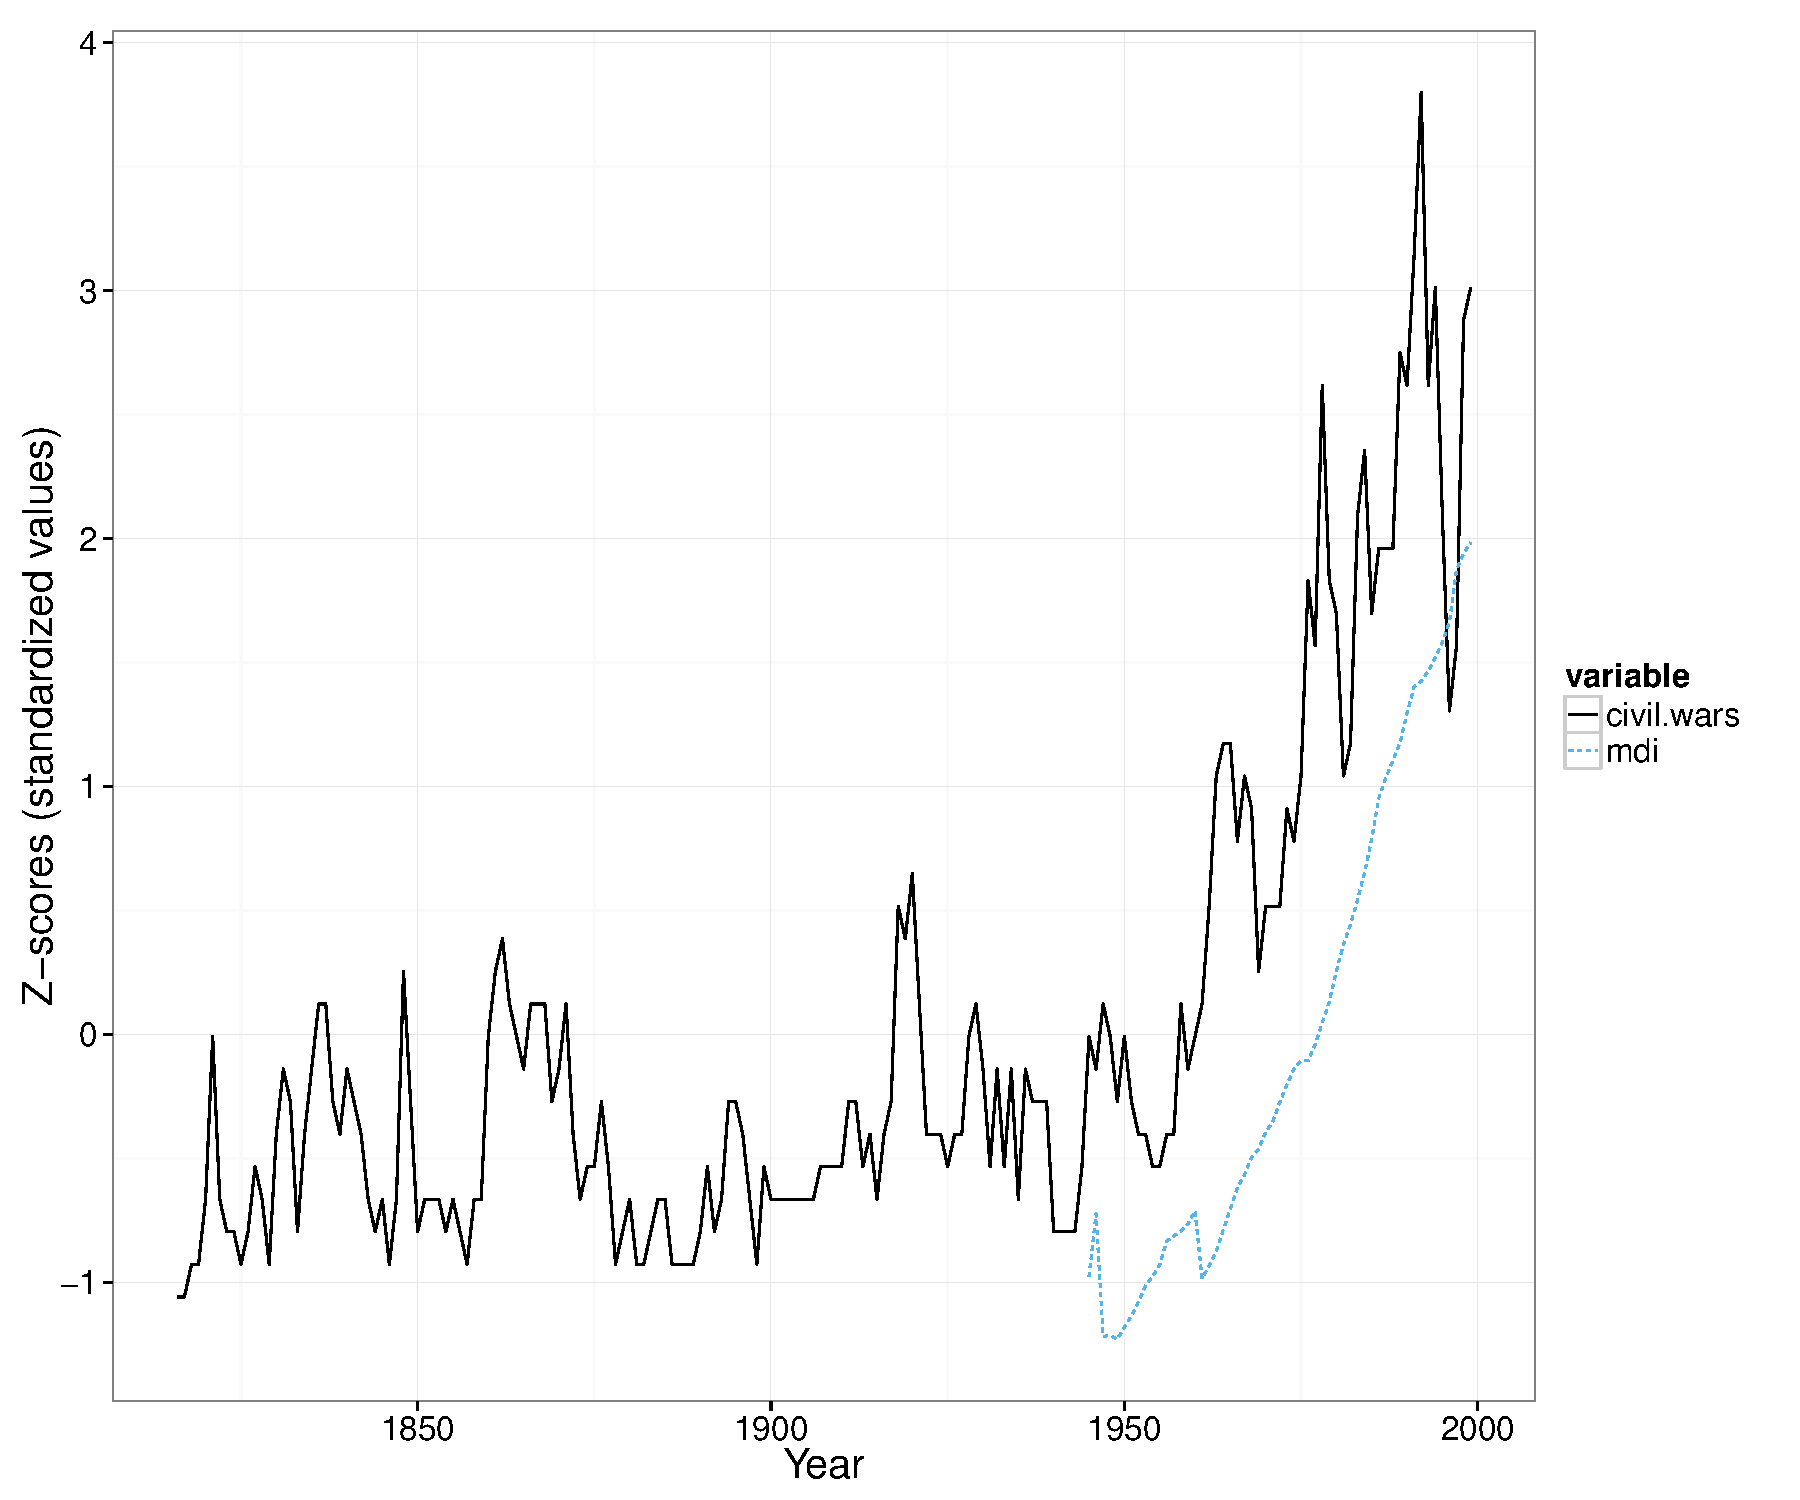
\includegraphics{./media_civil_war_files/figure-markdown/globalplot.pdf}
\caption{Mass Media Density and Civil Wars Globally, 1816-1999}
\end{figure}

This research note advances a novel theoretical proposition on the
relationship between mass media and civil war which accounts for
previous qualitative findings of mass media fomenting civil war onset
and recent quantitative evidence that mass media decrease the
probability of civil war onset (Warren). Paradoxically, it is precisely
because dense mass media systems strengthen the state that the first
appearance and early spread of mass media within a country should
\emph{encourage} insurgencies. When mass media spreads enough within a
country to constitute a mass communications system, this triggers
communicative economies of scale which so increase the payoffs of
controlling the state that it incentivizes violent insurgency before the
\emph{ex ante} holders of state power become normatively locked-in and
effectively impossible to challenge.\footnote{As discussed below, beyond
  a certain threshold of mass media the probability of observing a civil
  war is effectively zero.} A key point of my account, however, is that
the economies of scale peculiar to information production within a mass
communications system represent a qualitative change which occurs only
at a certain threshold of mass media density. This is why there is an
inflection point at which the effect of mass media should change from
positive to negative at a certain point in its range. The
counter-intuitive implication is that the very pacifying effect of a
mass communications system charges the early spread of mass media with a
bellicose effect until the threshold of mass communications is crossed.

To compare the non-linear ``war before peace'' theory to the linear,
general pacification theory, I generate causal leverage by deducing
three new observable implications at two levels of analysis, within and
outside the original sample used in the most recent and systematic study
on this question (Warren 2014). I use a combination of traditional
parametric and semi-parametric regressions to compare linear and
non-linear model fits on the original sample. (MENTION EFFECT SIZE HERE)
I then explore the composition of this effect by disaggregating the
specific information-communication technologies of television,
newspaper, and radio (MENTION EFFECT SIZE HERE). I then consider
long-term historical time-series at the international level, to examine
whether the non-linear theory helps explain the broad empirical pattern
of civil war prevalence at the international level. (MENTION EFFECT SIZE
HERE)

The implications of this research note are two-fold. First, it
contributes to the project of building ``rich theory'' for the new and
burgeoning research agenda on the ICT and political conflict nexus (CITE
LYALL AND DEFOE), demonstrating in particular the importance of
non-linearities in political conflict research. Second, it contributes
novel quantitative evidence helping to explain the severity and timing
of one of the most lethal dynamics in the world since World War II: the
exponential increase in civil wars around the world beginning in the
middle of the 1950s (CITE if possible).

This research note proceeds as follows. The first section provides a
brief summary and critique of the general pacification theory, providing
the basic rationale for why we should expect the relationship between
mass media and civil war onset to be non-linear. The second section
states the non-linear ``war before peace'' theory and deduces one
testable hypothesis which is mutually exclusive with the general
pacification theory and two which are not predicted by the general
pacification theory. The third section explains the data sources,
variables, and modeling strategy. A fourth section discusses the results
and a fifth section concludes.

\section{A Critique of the General Pacification Theory of Mass Media and
Civil
War}\label{a-critique-of-the-general-pacification-theory-of-mass-media-and-civil-war}

Many scholars of the modern nation-state have argued that by allowing
political elites to communicate with subjects across large territories,
the emergence of mass media technologies were a crucial condition for
the emergence of the modern nation-state (Anderson 1983; Deutsch 1953).
Within this tradition, contemporary political scientists often
conceptualize mass media technologies as instruments which increase the
state's ``soft power'' to induce loyalty and symbolic attachments (R. O.
Keohane and Nye Jr 1998; Nye Jr 1990, 168--69, 2004, 47--48). Issuing
from this perspective, one article from a recent issue of
\emph{International Organization} argues that precisely by increasing
the state's communicative power, mass media deter potential insurgencies
and therefore decrease the probability of civil war onset (Warren 2014).

According to Warren, technologies such as televisions, radios, and
newspapers decrease the probability of civil war onset because they
increase the state's communicative powers to induce loyalty from the
population more than they empower potential challengers of state power.
While mass media technologies lower the costs of communication for the
state and potential challengers alike, mass media technologies increase
the normative influence of the state in particular because of economies
of scale which are unique to the production of normative influence.
Because a media message achieves a larger effect on receivers who
believe the message was widely disseminated, the production of normative
influence through mass media brings increasing marginal returns for each
additional unit of effort, as each additional recipient receiving the
message increases the effect of the message on the rest of the
receivers. Because the state is inherently a larger-scale producer of
symbolic content than potential insurgent groups, Warren argues, higher
levels of mass media will be associated with normatively stronger states
and therefore lower probabilities of observing civil war.

Using state-level data for a large panel of countries from 1945 to 1999,
Warren demonstrates that, after controlling for other predictors of
civil war, mass media density (televisions, radios, and newspapers per
person) is associated with more than a tenfold decrease in the
likelihood of observing civil war in a particular country-year.

Although Warren shows that many statistical tests are consistent with
this general pacification theory, it is both empirically and logically
puzzling. First, if mass media density decreases the likelihood of civil
war as strongly and robustly as Warren argues, one might expect the
global proliferation of mass media since the 1950s to be followed by a
corresponding decrease in the global prevalence of civil war. It is
therefore puzzling that in the postwar period, the international
system's most rapid and widespread proliferation of mass media density
has coincided with its most dramatic increases in civil war. This
apparent contradiction does not inherently falsify the general
pacification theory, for of course it is possible that other drivers of
civil war onset have simply outweighed the pacifying effect of mass
media. Nonetheless, that an exponential increase in civil wars around
the world coincides so closely with an exponential increase in mass
media density raises the possibility that the effect of mass media on
civil war onset is not as simple as the general pacification theory
suggests.

The empirical patterns of mass media and civil war at the international
level point to two logical shortcomings in the general pacification
theory. The first shortcoming is that, while there should be increasing
marginal returns to the production of normative influence in the context
of \emph{mass communications,} there should not be a linear, one-to-one
relationship between a country's mass media density and its capacity for
mass communications (CITE SOMETHING ON MASS COMMS TIPPING POINTS). When
only a very small proportion of the population has access to mass media
technologies, those technologies do not imply the presence of a mass
communications system at merely low levels; they imply a country which
still categorically lacks the infrastructural capacity for properly mass
communications.\footnote{Of course, there is no way to know \emph{a
  priori} how many people need access to mass media technologies before
  they constitute a mass public network and therefore the categorical
  presence of a mass communications system. In any event, the question
  is pursued empirically below. At this stage, it suffices simply to
  note the contention that very low levels of mass media density do not
  reflect the positive presence of a mass communications capacity.} If
only a very small proportion of a population has access to television,
radio, or a newspaper, recipients of mass media messaging will know that
the vast majority of others will not be affected by the message. Thus,
within the subset of countries characterized by very low levels of media
density, the normative influence of messages delivered by mass media
technologies should not be enhanced by increasing marginal returns as
these are contingent on the recipient believing the message to be
\emph{widely} spread.

Mass media density only captures the reach of mass communications within
a particular country beyond the threshold at which mass media
technologies are sufficiently widespread to effectively consititute a
mass public network.\footnote{I assume throughout that mass media
  typically first appears within countries at very low levels relative
  to the population (low media density). I also assume throughout that,
  despite variable rates of change and short-run decreases, media
  density has a long-run tendency to increase. In other words, I assume
  that the dynamics of media density are non-stationary and trend
  upward. The Levin-Lin-Chu (2002) and Im-Pesaran-Shin (2003) tests for
  stationarity in panel data fail to reject the null hypothesis that
  media density is non-stationary (p = 0.75 and p = 0.1, respectively).
  See the Appendix for details.}

The second shortcoming is that if the level of mass media \emph{in
general} increases state strength as Warren argues, then for this very
reason, the \emph{first appearance and early growth} of mass media
within a country should increase the utility of controlling the state
relative to other means of merely influencing it. Especially given that
mass media density is non-stationary and trends upward in every country
in which it has been introduced, the first appearance of mass media
technology should increase the incentives of opposition groups to risk
insurgency before the development of a mass communications system
significantly increases the power of the incumbent and decreaes the
power of opposition groups outside the state. Additionally, the closer a
country's mass media density is to the threshold at which it will
constitute a capacity for mass communcations, the more attractive it
will be for opposition groups outside the state to gain control of the
state. It is increasingly urgent as the state becomes nearer to
consolidating its normative domination via mass communications and
therefore significantly less vulnerable to insurgency; also, the closer
the country is to the threshold the less time will a successful
insurgency be vulnerable to yet another insurgency before it
consolidates its own normative consolidation via mass communications.
Thus, if it is true that increasing mass media density makes state power
increasingly safe from insurgency, then before media density crosses the
threshold of constituting mass communications power, \emph{each
increase} in mass media density should further increase the payoffs to
violent insurgency.

\section{A Non-Linear Theory of Mass Media and Civil
War}\label{a-non-linear-theory-of-mass-media-and-civil-war}

Based on the implications of the previous section, this research note
advances a crucially modified theory of the relationship between mass
media technology and civil war: while high levels of mass media density
should indeed decrease the likelihood of civil war by increasing state
power and deterring insurgents, for this very reason the
\emph{introduction and early growth} of mass media density within a
country should \emph{increase} rather than decrease the likelihood of
civil war. Precisely because a capacity for mass communications
increases state power and becomes a robust deterrent against insurgents,
but low levels of mass media density do not yet constitute that power,
year-to-year increases in mass media density up to a certain threshold
should be positively associated with civil war onset.\footnote{It stands
  to reason that the same logic characterizes the incentives of
  incumbents, as each increase in mass media density up to that
  threshold also increases the utility of defeating insurgencies
  relative to stepping down or sharing power, thus further predicting
  civil war onsets. Yet the calculus of incumbents is likely more
  complicated given that under certain conditions it could be preferable
  to share the state's new mass communications power rather than risk
  losing it. At present, I focus on the calculus of insurgents and leave
  the calculus of incumbents to future research.} It is only beyond that
threshold that Warren's finding of a negative relationship between mass
media density and civil war should hold.

To test whether this modified theory is preferable to Warren's
attractively parsimonious theory, I pursue a strategy of increasing
causal leverage relative to the original analyses (G King, Keohane, and
Verba 1994, 30). A first strategy to increase causal leverage is to
deduce from the modified theory additional observable implications
exclusive to the modified theory, which expose the modified theory to
new opportunities for falsification.

Thus, I deduce three distinct observable implications of the modified
theory which either contradict the original theory or are not implied by
the original theory. If the modified theory is correct, then each of the
following should be true:

\textbf{Observable Implication 1:} There should exist a threshold of
mass media density below which year-to-year increases in mass media
density \emph{increase} the probability of civil war. This implication
flows directly from the logical critique of the original theory: If a
system of mass communications constitutes a significant increase in the
soft power of states and makes insurgency significantly more difficult,
then every increase in mass media density (the dynamics of which are
non-stationary and upward-trending) incentivizes insurgency without yet
increasing the risks.

\textbf{Observable Implication 2:} Because newspaper and television
production are subject to more significant economies of scale and higher
fixed costs than radio production, increases in newspaper and television
density should be more strongly associated with civil war onset than
increases in radio density before the threshold of mass
communications.\footnote{While these technologies are equally subject to
  economies of scale in their ``symbolic''" production (each additional
  message communicated decreases the cost of convincing another person
  of the message), here I refer to traditional or material economies of
  scale in the concrete production processes.} While each newspaper and
television production requires subsantial technological and logistical
investment the average costs of which decrease with scale, radio
productions are far less technologically and logistically costly and
therefore do not benefit as much from scale. The substantive political
implication of this difference is evidenced by historically and
geographically widespread examples of anti-state radio projects but far
fewer instances of anti-state television or newspapers with mass
audiences. While semi-illegal ``underground'' newspapers have been
historically and geographically widespread, the significant economies of
scale in newspaper production are such that they are almost always
limited to very limited circulation. After the threshold of mass
communications, the state's soft power increases more from mass
newspaper and television audiences than mass radio audiences, because
the economics of radio make mass radio audiences comparatively more
contestable by resource-poor challengers. Note that year-to-year
increases in radio density should still be positively associated with
the likelihood of civil war as radio production is still subject to
material and symbolic economies of scale which nonetheless will
privilege the state after the threshold of mass communications is
crossed, however less significant they are in comparison to newspaper
and television production.

\textbf{Observable Implication 3:} Given that mass media density
increased markedly after World War II from near-zero levels as measured
at the international level, year-to-year increases in mass media density
at the international level should be associated with increases in the
quantity of civil wars at the international level. On the contrary, if
the general pacification theory is correct, then year-to-year increases
in media density around the world should be associated with a decrease
in civil war onsets, controlling for other determinants of civil war
onset. Note, however, that the war-before-peace theory is consistent
with the general pacification theory in the expectation that mass media
density in the long run has a pacifying effect on the likelihood of
civil war onset, after controlling for the bellicose implications of
year-to-year changes.

\section{Data and Method}\label{data-and-method}

This section outlines the data, method, and overall analytical strategy
designed to weigh the general pacification theory (levels of mass media
density monotonically decrease the likehlihood of civil war onset) with
the war-before-peace theory (early increases in mass media density
increase the likelihood of civil war before levels of mass media density
decrease it in the long-run). As already discussed, the first feature of
the research strategy was to deduce distinct observable implications of
the new, competing hypothesis, at multiple levels of analysis, which
contradict or are not implied by the original hypothesis. This section
first details the data and methodological strategy for testing the first
two observable implications, and then considers separately the data and
methodological strategy for testing the third implication at the
international level.

The first two stages of analysis for the first two observable
implications use the replication data from Warren (2014), a panel
dataset of country-level variables covering 0 countries over a maximum
of 55 years in the period 1945-1999. As the variables used in the
present analyses follow the original analyses as exactly as possible,
for the sake of consistency and comparison, readers may consult the
original article for a more detailed discussion of the data. Briefly,
the dependent variable in all analyses is \emph{CIVIL WAR ONSET}, which
takes a value of 1 for all country-years in which a civil war begins and
zero otherwise. Civil wars are defined, following Sambanis (2004), as
any armed challenge to state sovereignty with explicit political
objectives, local recruits, and more than 500 deaths in the first year
or more than 1,000 deaths within the first three years. The main
indepdendent variable is \emph{MDI,} which captures overall mass media
density, or the total number of newspapers, televisions, and radios per
100 people. \emph{NEWSPAPER}, \emph{TV}, and \emph{RADIO} reflect the
number of each particular technology per 100 people. A battery of
control variables which are believed to be associated with civil war
onset include the following. \emph{OIL EXPORTER} takes a value of 1 if
greater than one-third of a country's total export revenus are from
fossil fuels. \emph{DEMOCRACY} is the traditional measure from the
well-known Polity IV data set, on a scale from 1-21.
\emph{DEMOCRACY\^{}2} is the square \emph{DEMOCRACY}, to control for the
possibility of non-linear effects. \emph{PEACE YEARS} counts the number
of years since a previous civil war, and a natural cubic spline of peace
years to control for temporal dependence. Finally, \emph{GDP PER
CAPITA}, \emph{ETHNIC FRACTIONALIZATION}, \emph{RELIGIOUS
FRACTIONALIZATION}, and logarithms for \emph{LAND AREA},
\emph{MOUNTAINOUS TERRAIN}, and \emph{POPULATION} complete the main
battery of controls dictated by previous research and employed in the
original analyses. Also following the original analyses, all independent
variables are lagged by one year.

Because observable implication 1 posits a threshold or tipping-point
beyond which the hypothesized effect of mass media changes direction, it
raises the question of how to test for the presence of such a threshold.
The typical procedure for testing the presence of curvilinear effects is
to include in regression analysis a polynomial of the independent
variable of interest; if both the linear term and the polynomial are
differently signed and significant, it is taken as evidence of a
curvilinear effect. The first problem with this convention is that it
does not effectively inform us about the thresholds for the independent
variable's heterogenous effects, and indeed is typically used as a
substitute for having to do so. More importantly, however, parametric
estimates can fail to detect important curvilinear effects (Fr{ö}lich
2006). On the other hand, nonparametric regressions are significantly
less theoretical and less parsimonious and therefore less valuable for
theory testing.

To balance these trade-offs, analysis begins with a combination of
simple graphical analysis and non-parametric regression to test for the
presence of a threshold at which the effect of mass media density
changes, and then traditional parametric regressions will provide
additional tests and more convenient estimates of effect sizes.
Graphical analysis is used to explore several features of the
distributions of mass media density and civil war relevant to
understanding their relationship, discussion of which is postponed until
the analysis in the following section. To statistically test whether
mass media density has a non-linear effect on civil war onset, and to
gain further insight into the threshold at which mass media density
constitutes a mass communications system, a semi-parametric Generalized
Additive Model (GAM) is estimated such that the effect of mass media
density is estimated via nonparametric smooth but all other predictors
are estimated traditionally. Estimation via non-parametric smooth
basically allows for the maximum-likelihood estimate of a traditional
logistic regression to inductively identify curvature in the
relationship between the independent and dependent variable; the
smoothness of the curves is determined by penalized regression splines
which are themselves estimated to maximize likelihood. While the GAM
model with non-parametric smoothing is a well-established tool for
testing non-linear hypotheses, it is not readily interpretable and
inferentially problematic precisely because it lacks a parameter
(coefficient) which could straightforwardly represent a hypothesized
effect. Thus, a simple analysis of variance (ANOVA) is used to test
whether a non-linear fit of mass media density better explains variation
in civil war onset than a linear fit; and graphical visualization of the
smooth terms will be used to further understand the threshold at which
mass media density constitutes a mass communications system. If a
non-linear fit of mass media density is superior to a linear fit and the
graphical inspections reveal a non-trivial subset of civil war onsets
increasing in mass media below an identifiable threshold at which mass
media density is robustly associated with decreasing probability of
civil war, then we will consider observable implication 1 to be
tentatively confirmed and the subsequent analyses will be informed by
these preliminary analyses.

To further explore observable implication 1 and test oservable
implication 2, the analysis replicates a baseline model from Warren's
original analysis (2014) and tests whether the pacification effect is
observed even within the subset of country-years characterized by mass
media density levels below the threshold (if any) identified in the
first analyses. If observable implication 1 is shown to be consistent
with the data in the first stage of analyses, it will be expected that
the pacification effect of mass media density will not hold within the
subset of country-years below the threshold at which it constitutes a
mass communications system. On the contrary, the expectation advanced by
the war-before-peace theory is that year-to-year increases in mass media
density will \emph{increase} the likelihood of civil war onset rather
than decrease it. Observable implication 2, which predicts that the
bellicose effects of mass media density should be greatest for newspaper
and television density compared to radio density, is examined by
additional regression analyses which disaggregate the indepedent
variable of mass media density into its component parts. Observable
implication 2 will be affirmed if the coefficients for newspaper and
television density are greater than and statistically distinguishable
from the coefficients for radio density.

Observable implication 3 seeks causal leverage from a level of analysis
distinct from the level at which the original theory was tested
(country-level). Additionally, observable implication 3 permits
examination of a substantially expanded historical range because for
many of the key variables data are available beginning from the early
nineteenth century. For the dependent variable, the Correlates of War
data provide a comprehensive record of all intra-state wars since 1816.
The Polity IV measure of democracy, discussed above, covers many
countries as far back as 1800 and is commonly used for
international-level estimates. For the other key determinant of civil
war onset, GDP per capita, the Maddison Project provides widely-used
estimates for all countries as far back as possible, in many cases
extending well before 1800 (Bolt 2013). Finally, while no general
measure of mass media density is available before 1945, I exploit a
pecularity of television diffusion to reliably and substantially extend
its time-series. Because the international mean for television density
is zero in the earliest two years available (1945 and 1946) and the
time-series of television density is an integrated (unit-root) process
which trends upward, the international mean for television density in
every year prior to 1945 is highly likely to be zero. Thus, I construct
an historically-extended international-level variable for \emph{TV}
equivalent to the one discussed above but which takes a zero for all
years prior to 1945.

To test observable implication 3, I estimate a series of regressions
using the negative binomial distribution for count data, where the
dependent variable is the total count of civil wars in the international
system. While the theoretical issues of time-series modeling of count
data are not negligible, a lagged dependent variable is conventiently
interpretable as a growth rate and adequately controls for
autocorrelation given an integrated dependent variable.

One drawback to this strategy is that several of the other control
variables in the main regressions are not available for such a long
historical period and their omission could lead to biased or spurious
estimates. Luckily, there are several good reasons why the threat of
omitted variable bias is outweighed by the leverage gained by testing
these hypotheses at the international-level and with an elongated
time-series. First, the variables related to physical geography such as
\emph{OIL EXPORTER}, \emph{LAND AREA} and \emph{MOUNTAINOUS TERRAIN} are
unlikely to vary appreciably because, while in principle they can vary
from changes in the number or size of states, they refer to quantities
which are ultimately fixed at the international level. Second, while
variables such as \emph{RELIGIOUS FRACTIONALIZATION} and \emph{ETHNIC
FRACTIONALIZATION} are likely to have varied since 1816, a far greater
proportion of their variance is likely to be cross-sectional and
therefore irrelevant to modeling civil wars at the international level.
Third, if one re-estimates the original models from the 1945-1999 period
with only the democracy variables and GDP per capita as the only control
variables, the estimates are not substantially different than the full
models with all controls, suggesting that time-series analysis excluding
these variables is still a credible strategy for hypothesis testing. The
fourth key reason why these risks of omitted variable bias are not
prohibitive is that the theoretical and subsantive gains of extending
the original sample to a long-run historical time-series analysis are
great: theoretically it is necessary because the arbitrarily truncated
nature of the original sample does not contain enough information
regarding the key relevant comparison (namely, the difference between
positive and zero mass media density), substantively because the most
politically salient and puzzling stylized fact about civil war is its
far greater prevalence in the period 1945-1999 \emph{compared} to the
previous period of modern world history.

Another drawback to this strategy is that considering only television
density apart from newspaper and radio density may fail to capture mass
media density in general. However, first, television density is highly
correlated with mass media density and disaggregated regressions in the
original analyses also show that television density has strong and
robust effects in the same, expected direction of mass media density.
Second, because television, with newspapers, is subject to greater
economies of scale than radio and is therefore more likely to be
pacifying, it should therefore be a relatively harder test of the
war-before-peace hypothesis than mass media density in general. If mass
media density truly has a monotonic pacifiying effect on the likelihood
of civil war rather than the non-linear effect hypothesized here, then a
long-run time-series analysis of television density should be more
likely to suggest monotonic pacification than mass media density in
general. If the war-before-peace implication is observed for television
density, it would be stronger evidence of the hypothesis than would be a
fuller measure of mass media density.

As robustness checks, subsequent models of the international-level
dynamics include controls for global events likely to shape the
likelihood of civil war onsets. \emph{WWI} is a dummy variable for the
years 1914-1918, \emph{WWII} is a dummy variable for the years
1939-1944, and \emph{Cold War} is a dummy variable for the years
1947-1991. Finally, to check that results are not dependent on the years
in which a value of 0 is imputed to televison density, I include the
variable \emph{IMPUTED} which is a dummy variable for all years before
1945. All dummy variables take a value of 1 when they are equal to the
condition they state, and a value of 0 otherwise.

\section{Analysis}\label{analysis}

To gain a better sense of the bivariate relationship between mass media
density and civil war onset, while keeping the distributions in
perspective, Figure 2 displays four violin plots.\footnote{The violin
  plot is a simple graphical device similar to the traditional boxplot
  but with a density trace (Hintze and Nelson 1998; Kastellec and Leoni
  2007).} The violin plots on the left display the distribution of mass
media density for all country-years in which there is no civil war
onset, while the violin plots on the left display the same distribution
for all country-years in which there is a civil war onset. The violin
plots in the top half of the figure are scaled by the total count of
cases for all country-years whereas the plots in the bottom half are
scaled with respect to the count of cases within each distribution. Each
plot contains three points which indicate the 25th percentile, median,
and 75th percentile within each distribution. These plots illustrate
three important facts about the distributions of civil war onset and
mass media density in this sample of countries between 1945-1999.

\begin{figure}[htbp]
\centering
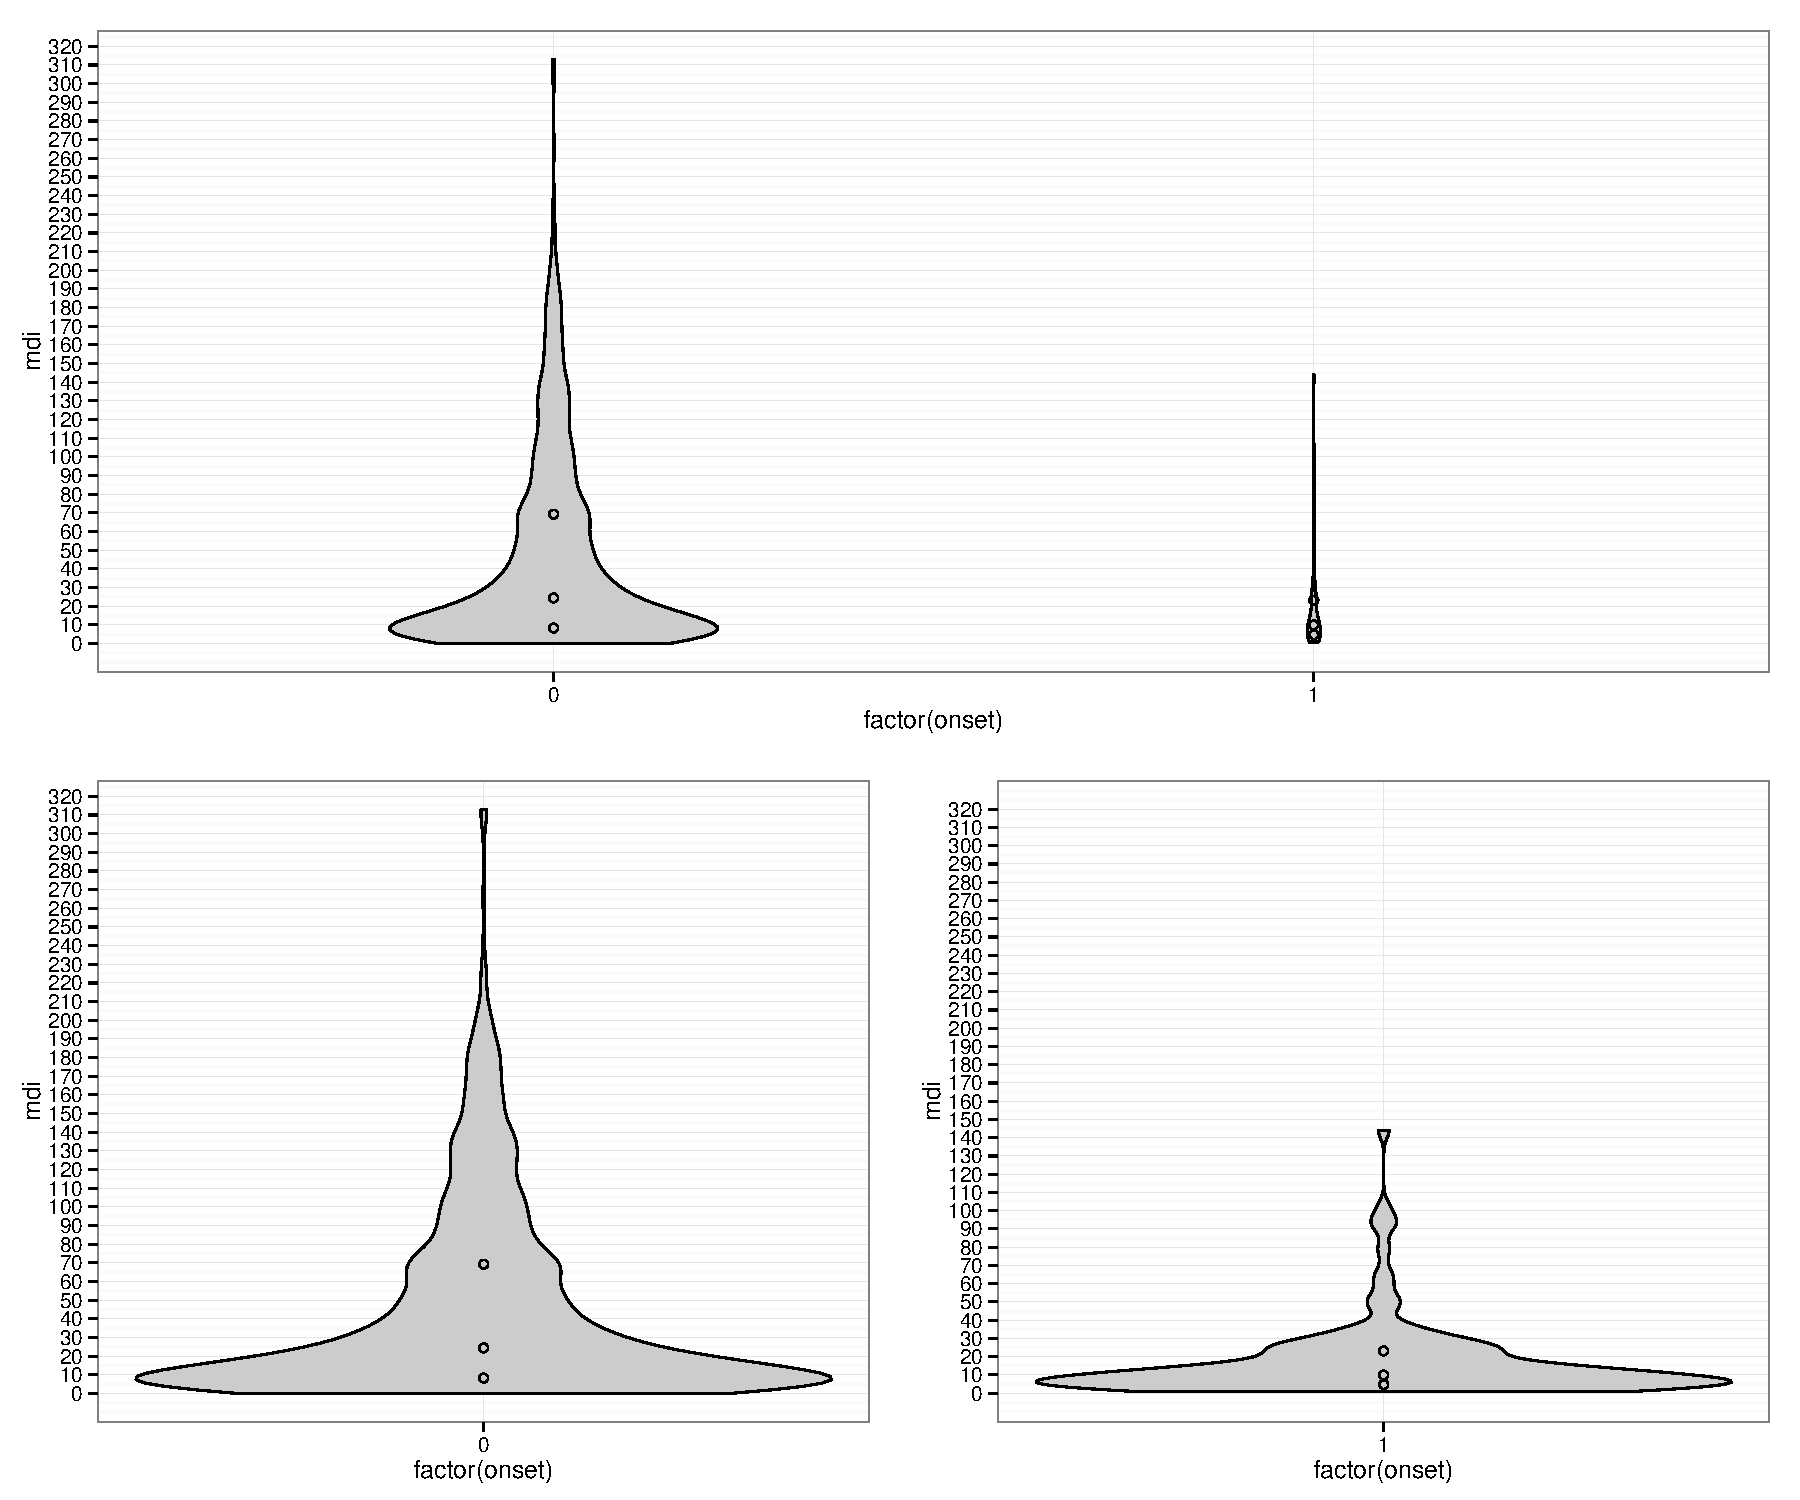
\includegraphics{./media_civil_war_files/figure-markdown/violinplot.pdf}
\caption{Violin plot of media density for all civil war onsets}
\end{figure}

First, these distributions challenge a key rationale for questioning the
qualitative evidence that mass media plays a causal role in generating
civil war onsets. Warren argues that those cases in which mass media are
known to have played a significant role in civil war--cases such as
Yugoslavia and Rwanda in the early 1990s (MDIs of 40.5 and 6.3,
respectively)--``unrepresentative cases\ldots{} characterized by unusual
levels of mass media weakness'' (Warren 2014, 132). Warren argues that
because analysts have effectively selected these cases on the dependent
variable, they ``observe mass communication behavior only in those
countries that are experiencing the outbreak of large-scale civil
conflict''(Warren 2014, 132). The implication is that the positive
association between mass media and civil war established by previous
qualitative research is ``spurious'' (132) and that ``expanding our
focus to the full universe of cases reveals quite a different picture''
(123).

Illustrating the entire distribution of the full universe of cases,
however, Figure 2 illustrates that cases such as Yugoslavia and Rwanda
are indeed fairly typical country-years in the period 1945-1999. While
it is true that in these cases mass media density is below the global
average \emph{in that year}, these cases bracket the global median of
MDI (37.03) by less than half of one standard deviation (8) on either
side. Thus, some of the well-known cases which illustrate the bellicose
effects of mass media are indeed highly representative of MDI levels
globally in the post-war period until 1999.

Second, if there is a problem of unrepresentativeness it is that the
extreme right-skew of MDI in peaceful country-years likely drives a
disproportionate amount of the negative association between levels of
MDI and civil war. Figure 2 illustrates that no civil war has ever been
observed in any country-year characterized by MDI greater than roughly
150, but that these are highly unrepresentative cases (in the 94\%
percentile). This is important because, as the following stage of
analysis will investigate more thoroughly, it indicates that the actual
relationship between mass media and civil war may be driven by a
minority of cases with uncommonly high values on the independent
variable, leading us to inferences which do not necessarily describe
most cases.

Finally, civil wars are most frequently observed at low but positive
levels of MDI, compared to the zero level. \emph{Prima facie} this is
contrary to what we would expect from the general pacification
hypothesis; if the relationship between MDI and civil war onset is
negative and monotonic, we would expect civil wars to be more frequent
at the zero level of mass media density. Rather, the distribution
suggests the possibility of non-linearity at low levels of mass media
density, precisely as predicted by the war-before-peace hypothesis. Of
course, some third variable could very well account for this apparent
non-linearity in the bivariate relationship. For this reason, the
following section turns to a statistical test of this non-linearity,
controlling for all of the other variables in the original model.

\subsection{Considering Non-Linearity with Semi-Parametric
Regression}\label{considering-non-linearity-with-semi-parametric-regression}

To test whether mass media density has a non-linear effect on civil war
onset, this section compares the fit of a baseline logistic regression
replicated from Warren (not displayed) with an additive semi-parametric
regression model identical in every respect except that the effect of
MDI is estimated with a nonparametric smooth allowing it to vary at
different levels of MDI. Specifically, I estimate the model

\[ Onset_{it} = \alpha + f_1 (LogMDI_{it}) + Controls_{it} \beta  + \varepsilon_i \]

where the partial-regression function $f_1 (\cdot)$ is fit by a
smoothing spline (Fox 2002; Wood 2000) and $CONTROLS_{it}$ is the vector
of control variables used in Warren's original models. The number of
smoothing splines is determined by generalized cross validation as part
of the estimation procedure.\footnote{The model was estimated using the
  function \emph{gam} in the \emph{mgcv} package for R.}

Figure 3 plots the value of the smooth terms for each level of the
logarithm of MDI, i.e.~the estimated effect of the logarithm of MDI on
the probability of civil war onset across its range. The result is
consistent with the war-before-peace hypothesis: MDI is positively
associated with civil war onset up to a threshold, the estimated effect
slightly increasing up to that threshold, before changing direction and
decreasing monotonically. To determine whether the non-linear fit is
superior to the linear fit, a simple analysis of variance (ANOVA) can be
used to contrast the deviance of each model. Table 3 displays the
results, which suggest that the non-linear fit reduces the deviance by
17.9 and is statistically significant.

\begin{figure}[htbp]
\centering
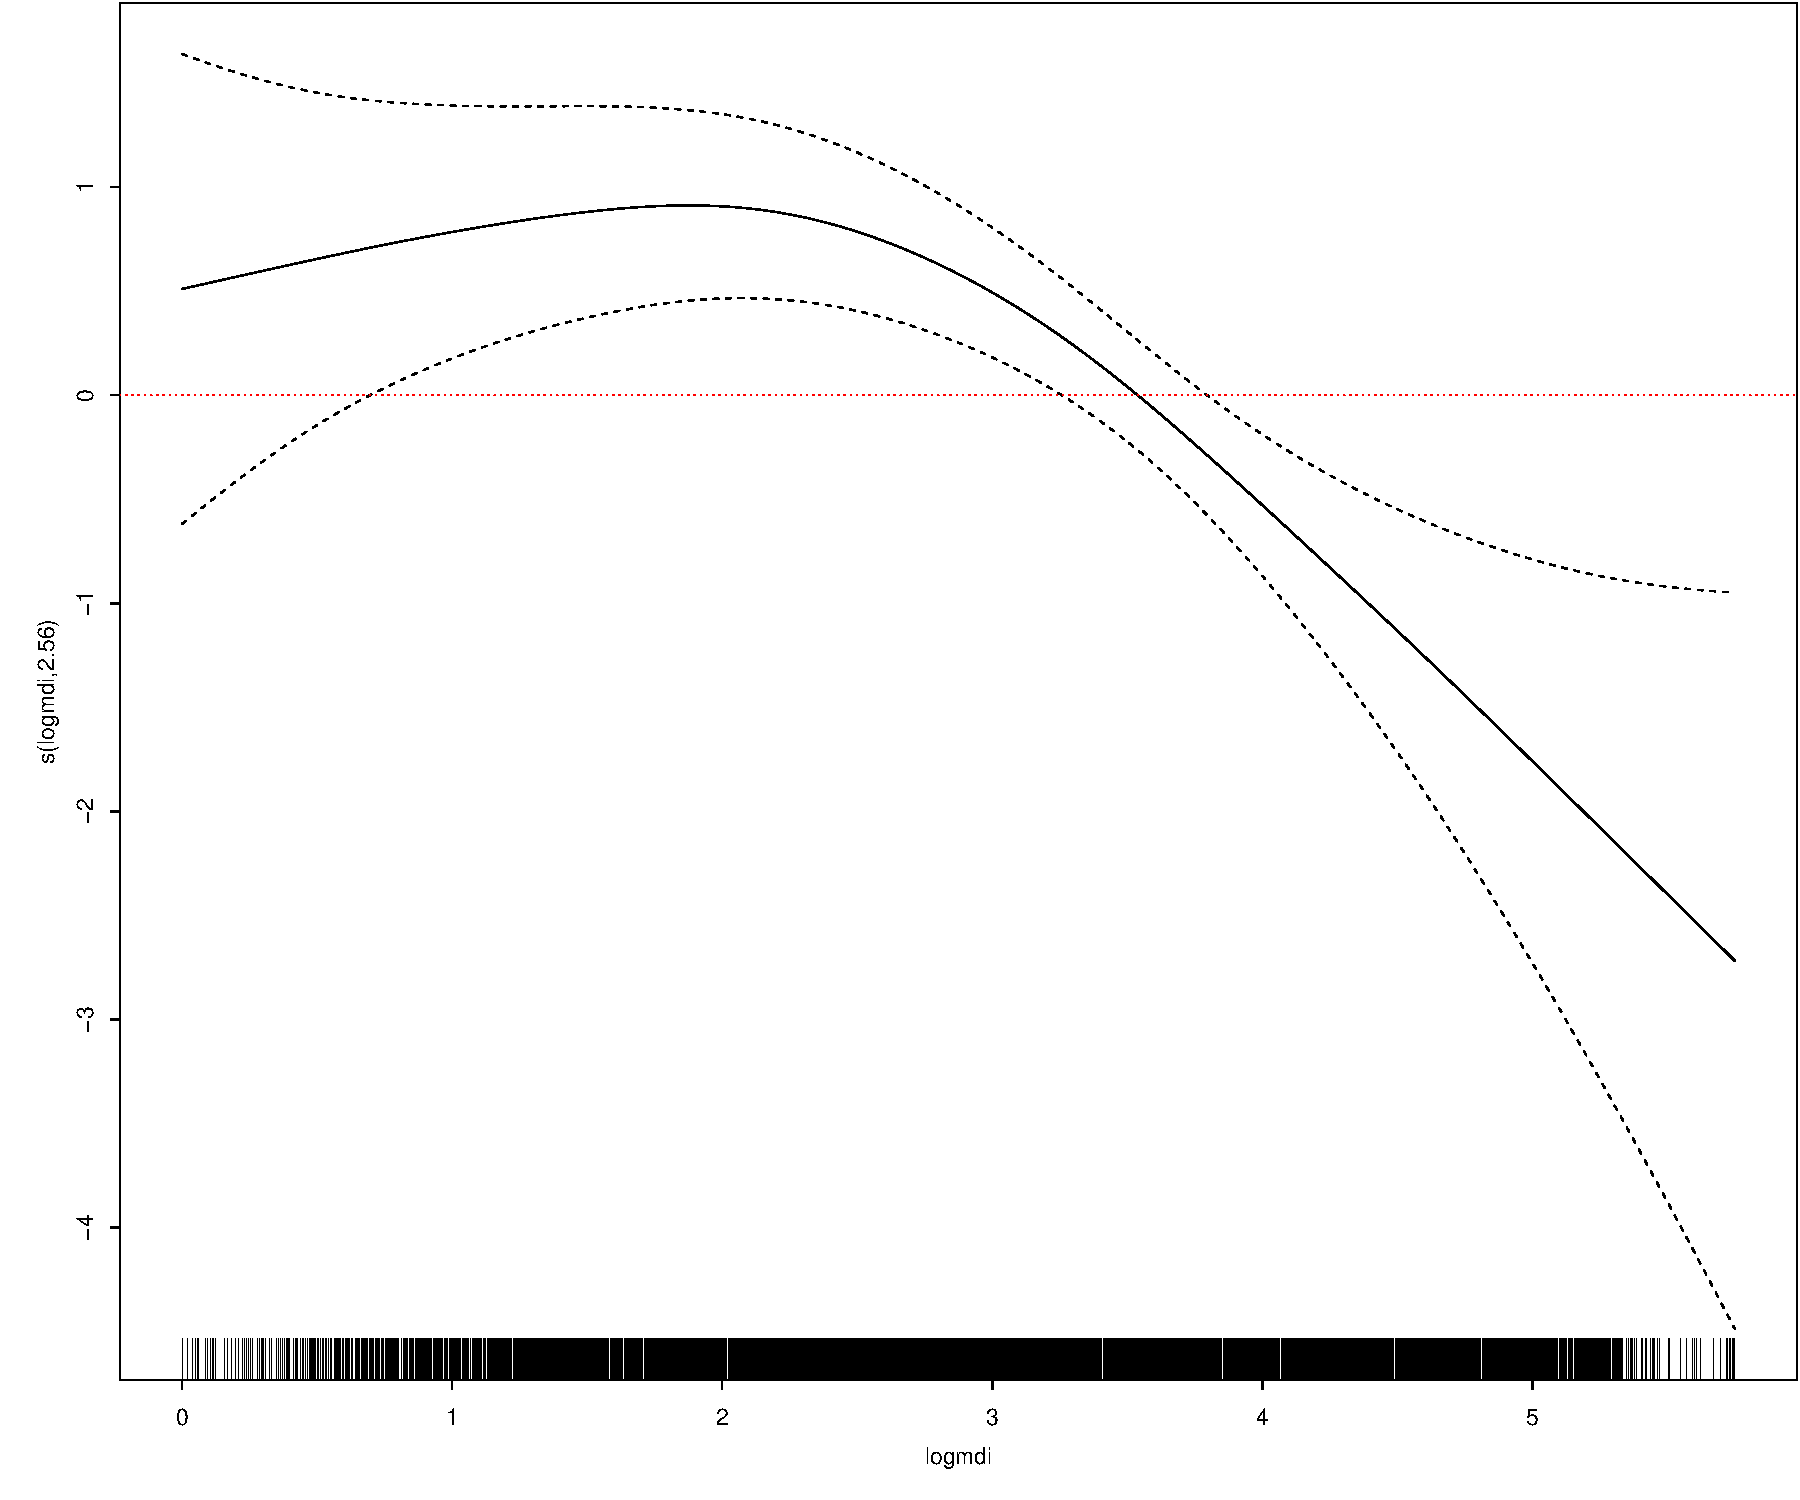
\includegraphics{./media_civil_war_files/figure-markdown/nonlinear-plot.pdf}
\caption{The Non-Linear Effect of MDI on Civil War Across Levels of MDI}
\end{figure}

\begin{table}[!htbp] \centering 
  \caption{ANOVA Comparing Linear and Non-Linear Effects of MDI on Civil War Onset} 
  \label{} 
\footnotesize 
\begin{tabular}{@{\extracolsep{5pt}} cccccc} 
\\[-1.8ex]\hline \\[-1.8ex] 
 & RESID. DF & RESID. DEV & DF & DEVIANCE & P-VALUE \\ 
\hline \\[-1.8ex] 
1 & $5,884$ & $1,070.00$ & $$ & $$ & $$ \\ 
2 & $5,882.00$ & $1,052.00$ & $1.60$ & $18.00$ & $0.0001$ \\ 
\hline \\[-1.8ex] 
\end{tabular} 
\end{table}

Due to the atheoretical nature of nonparametric regression and the
difficulty of drawing inferences from multiple smoothed terms, the
following section proceeds with traditional parametric logistic
regressions on subsets of the sample suggested by the semi-parametric
model. The second observable implication is also considered in the
following section.

\subsection{Estimating the Effect of Mass Media Density Before and After
the Threshold of Mass
Communications}\label{estimating-the-effect-of-mass-media-density-before-and-after-the-threshold-of-mass-communications}

To further test the hypothesis that MDI increases the likelihood of
civil war before it is sufficiently high to represent a mass
communications system (and to obtain a parsimonious estimate of the
effect size), I estimate a series of traditional parametric regressions.
I began by creating a subset of the original sample containing only
country-years with MDI levels below the inflection point identified by
the non-linear regression. Figure 2 suggests that the relationship
between MDI and civil war begins to change direction when the logarithm
of MDI is equal to about 2, which is an MDI level of about 6.38. While
it is reasonable to think such a low threshold might only correspond to
a substantively trivial number of cases, on the contrary, this subset
contained 1358 cases or about 20\% of the original sample. I estimate
traditional parametric regressions separately for each subset, all of
which are variations on the form

\[ Onset_{it} = \alpha + MDI_{it} \beta_1 + Controls_{it} \beta_2  + \varepsilon_{it}, \]

where all the variables are the same as in the previous equation, with
the exception that \emph{MDI} is not logged.

To ensure the robustness of the results, all of the models in this
section pertaining to this subset of pre-mass communications systems
were tested separately using a series of lower and higher cutoff values.
The main results reported below for changes in MDI under the threshold
of mass communications are consistent using a cutoff as low as 4 (13\%
percentile) and as high as 10 (27\% percentile).\footnote{See online
  appendix for full results.} To avoid ``cherry-picking'' a cutoff
within this range, the models below report results for the 25\%
percentile (MDI = 28.23), a conventional value for segmenting
distributions.

Table 1 shows coefficients and standard errors from several logistic
regressions modeling the determinants of civil war onset, with
adjustment for rare events (Gary King and Zeng 2001).\footnote{Traditional
  logistic regression estimated by maximum-likelihood would likely
  underestimate the probability of civil war onsets because civil wars
  begin in relatively very few country-years. There are 114 (2.01\%)
  onsets in the full sample and 53 (3.36\%) in the subset of low-MDI
  country-years.} Before analysis, I subtracted the mean from each
continuous independent variable and then divided it by two standard
deviations so that all resulting coefficients are readily
comparable.\footnote{For continuous independent variables, the
  coefficient indicates the change in log-odds of a civil war beginning
  due to a two standard deviation increase from the mean of the
  independent variable; for dichotomous variables, the coefficient
  reflects the change in log-odds of a civil war beginning due to a
  change from 0 to 1 on the dichotomous variable, which is roughly
  equivalent to a two-standard deviation change in a continuous variable
  (``Scaling Regression Inputs by Dividing by Two Standard Deviations''
  2008).}

The first two columns of the following table display the results of a
baseline model which replicates Warren's original findings (Model 1) and
the same model estimated on the subset of country-years below the median
level of MDI (37.03). While Model 1 successfully replicates Warren's
main finding with a negative and statistically significant coefficient
for MDI levels, Model 2 indicates that this coefficient is not
statistically significant for country-years below the median level of
MDI. The second two columns estimate models nearly equivalent to the
first two but only for country-years below the 25th percentile of MDI,
roughly the inflection point suggested by the semi-parametric regression
estimated in the previous stage of analysis. Distinct from Models 1 and
2, the independent variables of interest in Models 3 and 4 are first
differences of media density ($X_{t} - X_{t-1}$), rather than levels of
MDI, for two reasons. First, by restricting attention to the 25th
percentile of media density, Models 3 and 4 are, in effect, already
controlling for the level of media density because they only include
units at a relatively similar (low) level of the independent variable.
Thus, level of media density would unlikely capture any causal effect,
positive or negative, which media density may exert on the likelihood of
civil war onset, whereas the first-differenced variable within this
subset effectively captures variations in national experiences of the
early spread of mass media.\footnote{The smallest year-to-year change
  within this subset is -5.43 and the maximum is 3.41.} In other words,
year-to-year differences are both substantively pertinent and
theoretically appropriate for testing the observable implications of the
hypothesis developed above.

The results suggest that Warren's general pacification theory would
significantly under-estimate the probability of civil war onset in
countries first observing the introduction and early spread of mass
media. Warren's baseline model (Model 1) would lead us to predict that a
country moving from zero MDI to the 25th percentile (7.65) would, on
average, cause the probability of civil war onset to decrease negligibly
by -0.01, from an already low 0.03 to 0.03. However, when we estimate
the same model on only those country-years in the 25th percentile of
mass media density (Model 3), we would predict that an increase of 7.65
would cause the probability of civil war onset to increase by an average
of 0.52, from 0.02 to 0.54.

\begin{table}[!htbp] \centering 
  \caption{Early Growth of Media Density Compared to Media Density in General} 
  \label{} 
\scriptsize 
\begin{tabular}{@{\extracolsep{5pt}}lcccc} 
\\[-1.8ex]\hline \\[-1.8ex] 
 & Warren & < Median MDI & \multicolumn{2}{c}{< 25th Percentile MDI} \\ 
\\[-1.8ex] & (1) & (2) & (3) & (4)\\ 
\hline \\[-1.8ex] 
 MDI & $-$2.50$^{***}$ & $-$2.00 &  &  \\ 
  & (0.71) & (1.50) &  &  \\ 
  $\Delta$MDI &  &  & 0.43$^{*}$ &  \\ 
  &  &  & (0.25) &  \\ 
  $\Delta$NEWSPAPER &  &  &  & 0.26 \\ 
  &  &  &  & (0.32) \\ 
  $\Delta$RADIO &  &  &  & 0.30 \\ 
  &  &  &  & (0.25) \\ 
  $\Delta$TV &  &  &  & 0.40$^{*}$ \\ 
  &  &  &  & (0.22) \\ 
  GDP PER CAPITA & $-$0.23 & $-$0.08 & $-$0.77$^{*}$ & $-$0.78$^{*}$ \\ 
  & (0.37) & (0.42) & (0.40) & (0.40) \\ 
  AREA & $-$0.39 & $-$0.37 & 0.10 & 0.01 \\ 
  & (0.33) & (0.36) & (0.48) & (0.48) \\ 
  MOUNTAINOUS & 0.49$^{**}$ & 0.49$^{*}$ & 0.34 & 0.37 \\ 
  & (0.25) & (0.26) & (0.39) & (0.40) \\ 
  POPULATION & 0.86$^{***}$ & 0.89$^{***}$ & 0.75$^{*}$ & 0.80$^{*}$ \\ 
  & (0.26) & (0.27) & (0.41) & (0.42) \\ 
  OIL EXPORTER & 0.83$^{***}$ & 0.62$^{*}$ & 1.30$^{***}$ & 1.30$^{***}$ \\ 
  & (0.28) & (0.32) & (0.49) & (0.50) \\ 
  DEMOCRACY & 3.10$^{***}$ & 2.50$^{*}$ & 2.70$^{*}$ & 2.50 \\ 
  & (1.20) & (1.30) & (1.50) & (1.50) \\ 
  DEMOCRACY$^2$ & $-$2.90$^{**}$ & $-$2.30$^{*}$ & $-$2.20 & $-$2.00 \\ 
  & (1.20) & (1.40) & (1.40) & (1.50) \\ 
  ETHNIC FRAC. & 0.11 & 0.17 & $-$0.43 & $-$0.38 \\ 
  & (0.22) & (0.23) & (0.35) & (0.36) \\ 
  RELIGIOUS FRAC. & 0.62$^{***}$ & 0.62$^{**}$ & 0.40 & 0.47 \\ 
  & (0.23) & (0.25) & (0.36) & (0.36) \\ 
  PEACE YEARS & $-$1.50 & $-$1.80 & $-$0.55 & $-$0.18 \\ 
  & (2.60) & (2.70) & (2.60) & (2.60) \\ 
  SPLINE 1 & 0.27 & $-$1.40 & 3.30 & 4.50 \\ 
  & (16.00) & (17.00) & (13.00) & (13.00) \\ 
  SPLINE 2 & $-$5.70 & $-$2.40 & $-$6.00 & $-$6.60 \\ 
  & (19.00) & (20.00) & (15.00) & (15.00) \\ 
  SPLINE 3 & 3.50 & 1.20 & 1.80 & 1.60 \\ 
  & (5.60) & (6.30) & (4.70) & (4.70) \\ 
  CONSTANT & $-$4.60$^{***}$ & $-$4.20$^{***}$ & $-$3.80$^{***}$ & $-$3.80$^{***}$ \\ 
  & (0.18) & (0.45) & (0.22) & (0.22) \\ 
 \textit{Observations} & 5,787 & 3,472 & 1,445 & 1,445 \\ 
\textit{Log likelihood} & $-$506.00 & $-$433.00 & $-$182.00 & $-$182.00 \\ 
\textit{Akaike information criterion} & 1,042.00 & 897.00 & 395.00 & 397.00 \\ 
\hline \\[-1.8ex] 
\textit{Notes:} & \multicolumn{4}{l}{$^{***}$p $<$ .01; $^{**}$p $<$ .05; $^{*}$p $<$ .1} \\ 
\end{tabular} 
\end{table}

While the difference between zero MDI and the 25th percentile 7.65 is a
useful yardstick with respect to the entire range of \emph{levels}
observed in the sample, the mean year-to-year change observed in the
subset of pre-mass communications systems is only 0.24 and the maximum
is only 3.41. Thus, to gain a more realistic sense of how the early
spread of mass media shapes civil war onset in the world, and to better
compare the substantive implications of the general pacification effect
with the war-before-peace effect, Figures 3 and 4 display the predicted
probability of civil war onset given different values of MDI levels and
year-to-year MDI changes across their historically observed ranges.

Considering all communications systems, the predicted probability of
civil war onset decreases from about .03 at the zero level of MDI to
roughly zero for any level of MDI greater than about 150, on average.
However, considering only pre-mass communications systems, a 3-point
change in MDI increases the probability of civil war onset from about
.03 to roughly .1, on average. Figures 3 and 4 also highlight the
essential assymetry of estimating negative versus postive effects on a
rare event. The pacifying effect of levels of MDI as identified by
Warren is an inherently small effect because the probability of
observing civil war onset is already very small in general. However, in
part, the size of the war-before-peace effect is notably larger and
represents a more politically salient risk for the same reason. Indeed,
because of this assymetry, it is within the 95\% confidence interval
that a 3-point change in MDI is associated with as much as a 30\%
increase in the probability of civil war onset.

\clearpage

\begin{figure} 
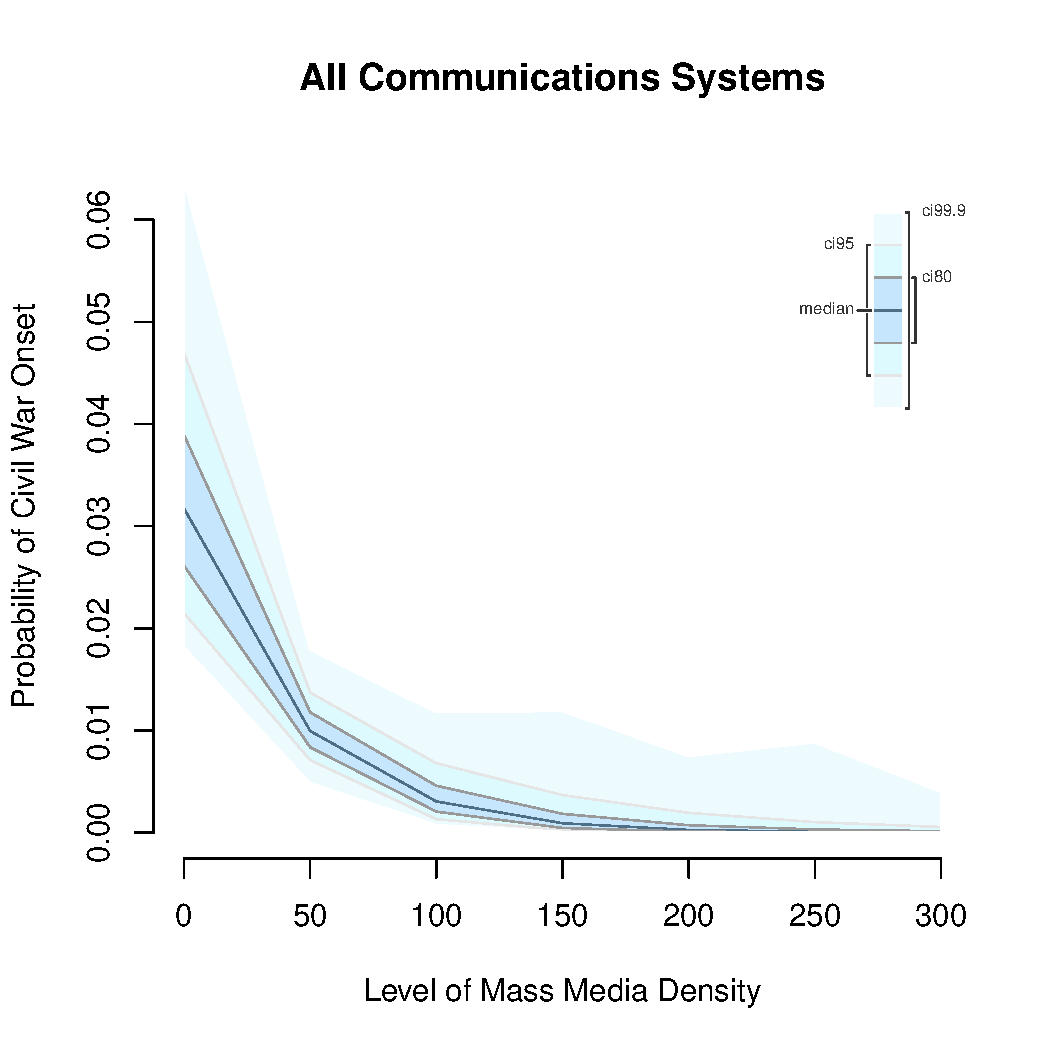
\includegraphics{figure/mdi_effect.pdf} 
\caption{Predicted probability of civil war onset given levels of media density} 
\label{myFigur} 
\end{figure}

\clearpage

\begin{figure} 
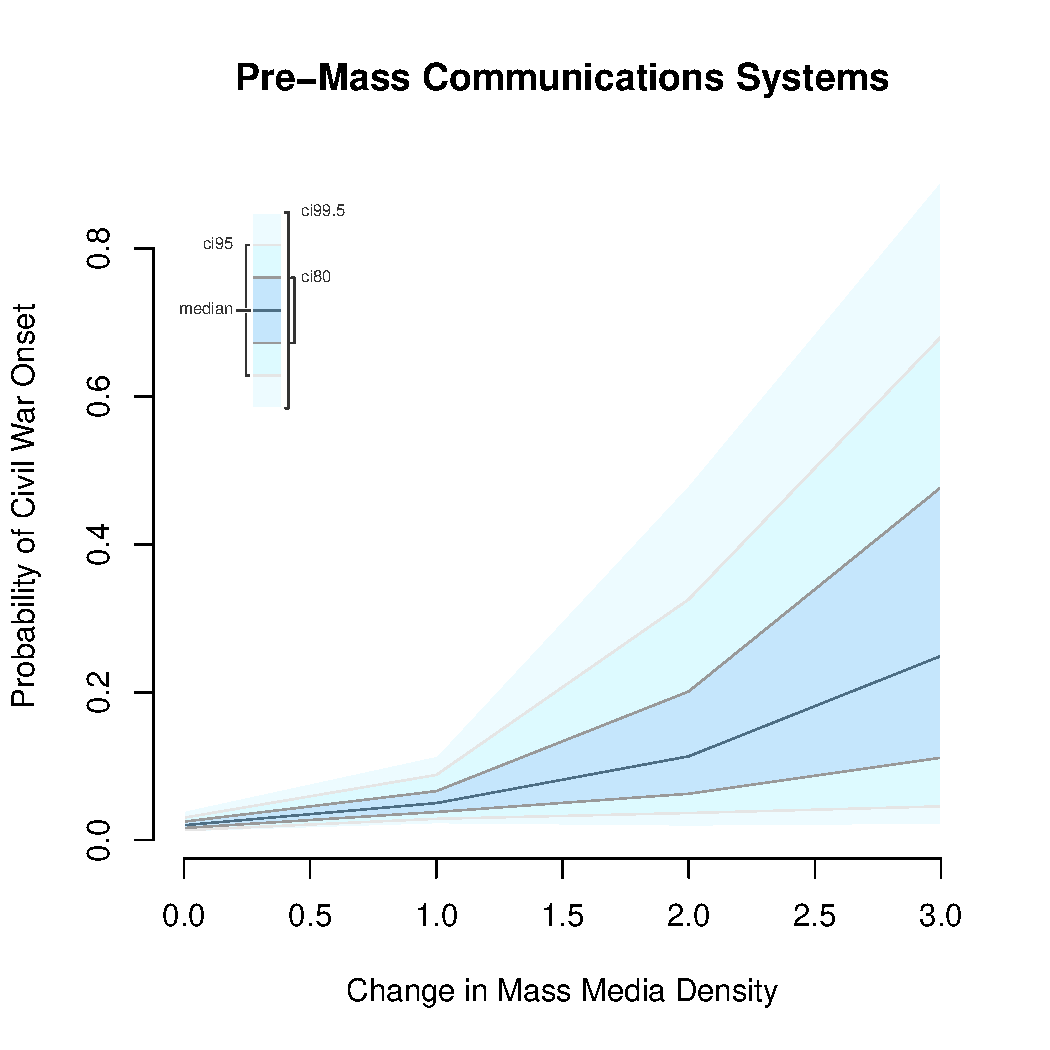
\includegraphics{figure/d_mdi_effect.pdf} 
\caption{Predicted probability of civil war onset given changes in media density} 
\label{myFigz} 
\end{figure}

To further assess the hypothesized mechanism, Model 4 considers the
separate effects estimated for each component of MDI (newspapers,
radios, and televisions per person), within the subset of pre-mass
communications systems. The results suggest mixed evidence of Observable
Implication 3, namely that television density should have the strongest
bellicose effect, whereas newspaper and radio density should have the
second and least strongest effects, respectively. Model 4 reveals that
controlling for each component, television does have the largest and
most statistically significant effect compared to newspaper and radio.
However, the model provides no evidence that newspaper or radio have any
independent effect.

\subsection{Mass Media Density and Civil Wars at the International
Level}\label{mass-media-density-and-civil-wars-at-the-international-level}

Table 4 models the number of civil wars in the international system
using the negative binomial distribution and lagged levels as well as
first differences of the number of civil wars on the right-hand side of
the equation. Model 1 is a baseline model. Column 2 includes controls
variables \emph{WW1}, \emph{WW2}, and \emph{COLD WAR.} Column 3 adds to
these the control variable \emph{IMPUTED.} Each model provides evidence
for Observable Implication 3, that with respect to the international
system in historical perspective, year-to-year increases in television
density are positively associated with the number of civil war onsets in
the second year. Figure 6 illustrates the expected change in global
civil war onsets for a range of changes in the global mean of television
density. These results are consistent with the evidence presented above,
reflecting that year-to-year increases in media density increase the
likelihood of civil war, even if media density has a pacifying effect in
the long-run. Interestingly, the international-level models do not
provide much evidence for the long-term pacifying effect, as the effect
is no longer statistically significant after controlling for \emph{WW1},
\emph{WW2}, and \emph{COLD WAR}. However, this could be for the simple
reason that global television density remains relatively low and has not
yet reached the threshold at which its pacifying effects would become
observable at the level of the international system.

\begin{figure}[htbp]
\centering
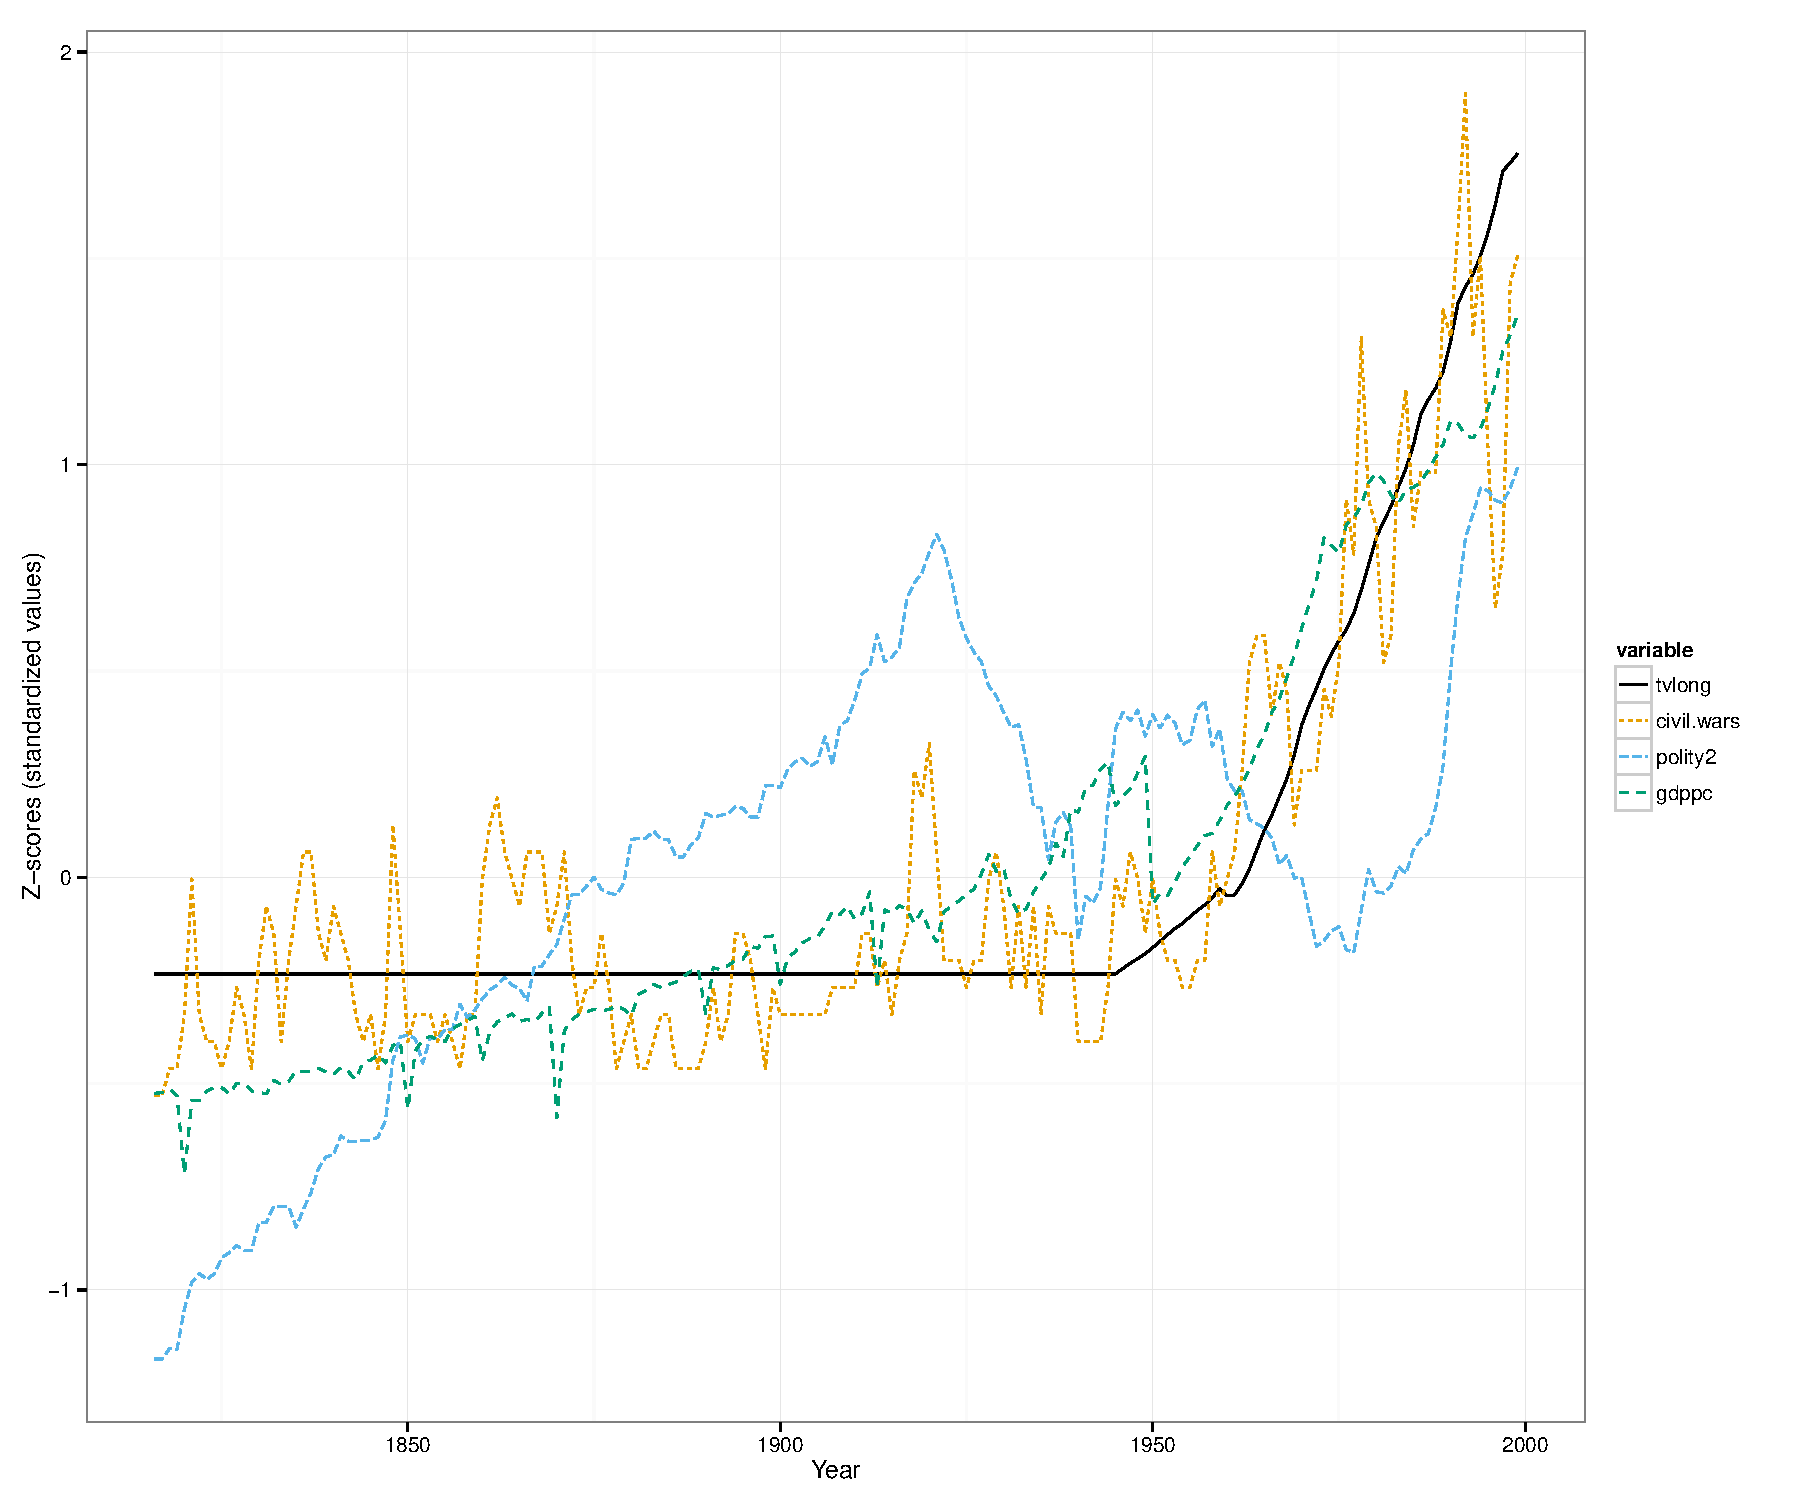
\includegraphics{./media_civil_war_files/figure-markdown/longrunplot.pdf}
\caption{TV, Democracy, Economic Growth, and Civil Wars Globally,
1816-1999}
\end{figure}

\begin{table}[!htbp] \centering 
  \caption{International-Level Regressions} 
  \label{} 
\scriptsize 
\begin{tabular}{@{\extracolsep{5pt}}lccc} 
\\[-1.8ex]\hline \\[-1.8ex] 
\\[-1.8ex] & \multicolumn{3}{c}{onsets} \\ 
\\[-1.8ex] & (1) & (2) & (3)\\ 
\hline \\[-1.8ex] 
 TV$_{t-1}$ & $-$0.80$^{***}$ & $-$0.53 & $-$0.43 \\ 
  & (0.30) & (0.35) & (0.34) \\ 
  $\Delta$TV & 0.36$^{**}$ & 0.46$^{***}$ & 0.51$^{***}$ \\ 
  & (0.14) & (0.15) & (0.15) \\ 
  GDP PER CAPITA$_{t-1}$ & $-$0.11 & $-$0.06 & $-$0.26 \\ 
  & (0.50) & (0.55) & (0.54) \\ 
  $\Delta$GDP PER CAPITA & $-$0.01 & $-$0.03 & $-$0.06 \\ 
  & (0.06) & (0.06) & (0.06) \\ 
  DEMOCRACY$_{t-1}$ & 0.20 & 0.86$^{***}$ & 0.89$^{***}$ \\ 
  & (0.16) & (0.22) & (0.22) \\ 
  $\Delta$DEMOCRACY & $-$0.21$^{**}$ & $-$0.21$^{**}$ & $-$0.25$^{***}$ \\ 
  & (0.09) & (0.09) & (0.09) \\ 
  DEMOCRACY$^2_{t-1}$ & 0.21 & 0.36$^{*}$ & 0.40$^{**}$ \\ 
  & (0.15) & (0.20) & (0.19) \\ 
  CIVIL WARS & 0.94$^{***}$ & 0.97$^{***}$ & 1.00$^{***}$ \\ 
  & (0.22) & (0.24) & (0.25) \\ 
  ONSETS$_{t-1}$ & 0.91$^{***}$ & 0.97$^{***}$ & 0.99$^{***}$ \\ 
  & (0.16) & (0.16) & (0.17) \\ 
  $\Delta$ONSETS & 0.16$^{***}$ & 0.17$^{***}$ & 0.17$^{***}$ \\ 
  & (0.02) & (0.02) & (0.02) \\ 
  YEAR & $-$0.09 & $-$0.93$^{*}$ & $-$0.77 \\ 
  & (0.39) & (0.55) & (0.53) \\ 
  WWI &  & $-$0.10 & $-$0.15 \\ 
  &  & (0.17) & (0.17) \\ 
  WWII &  & 0.43$^{**}$ & 1.50$^{***}$ \\ 
  &  & (0.22) & (0.33) \\ 
  COLD WAR &  & $-$0.88$^{***}$ & $-$0.96$^{***}$ \\ 
  &  & (0.20) & (0.20) \\ 
  IMPUTED &  &  & 1.20$^{***}$ \\ 
  &  &  & (0.34) \\ 
  CONSTANT & 0.53$^{***}$ & 0.56$^{***}$ & $-$0.24 \\ 
  & (0.04) & (0.08) & (0.25) \\ 
 \textit{Observations} & 182 & 182 & 182 \\ 
\textit{Log likelihood} & $-$260.00 & $-$257.00 & $-$256.00 \\ 
$\theta$ & 45,390.00  (485,212.00) & 45,395.00  (461,838.00) & 46,325.00  (469,369.00) \\ 
\textit{Akaike information criterion} & 544.00 & 544.00 & 545.00 \\ 
\hline \\[-1.8ex] 
\textit{Notes:} & \multicolumn{3}{l}{$^{***}$p $<$ .01; $^{**}$p $<$ .05; $^{*}$p $<$ .1} \\ 
\end{tabular} 
\end{table}

\clearpage

\begin{figure} 
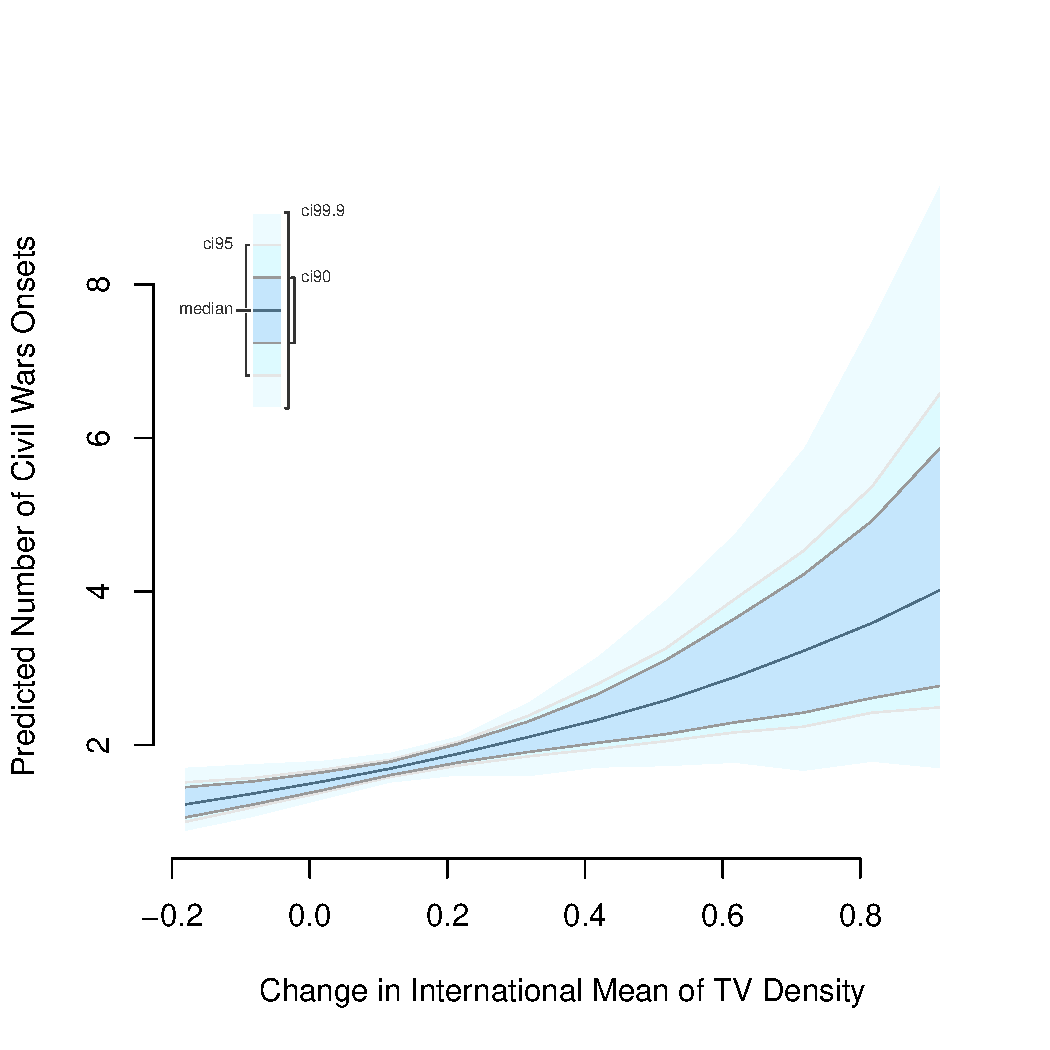
\includegraphics{figure/dtv_effect.pdf} 
\caption{Predicted number of civil war onsets given changes in global TV density} 
\label{myFigur} 
\end{figure}

\section{Supplementary Information}\label{supplementary-information}

\subsection{Contents}\label{contents}

\begin{enumerate}
\def\labelenumi{\arabic{enumi}.}
\itemsep1pt\parskip0pt\parsep0pt
\item
  Summary visualization
\item
  Tests of stationarity
\item
  Semi-parametric regressions on disaggregated media density
\end{enumerate}

\begin{figure}[htbp]
\centering
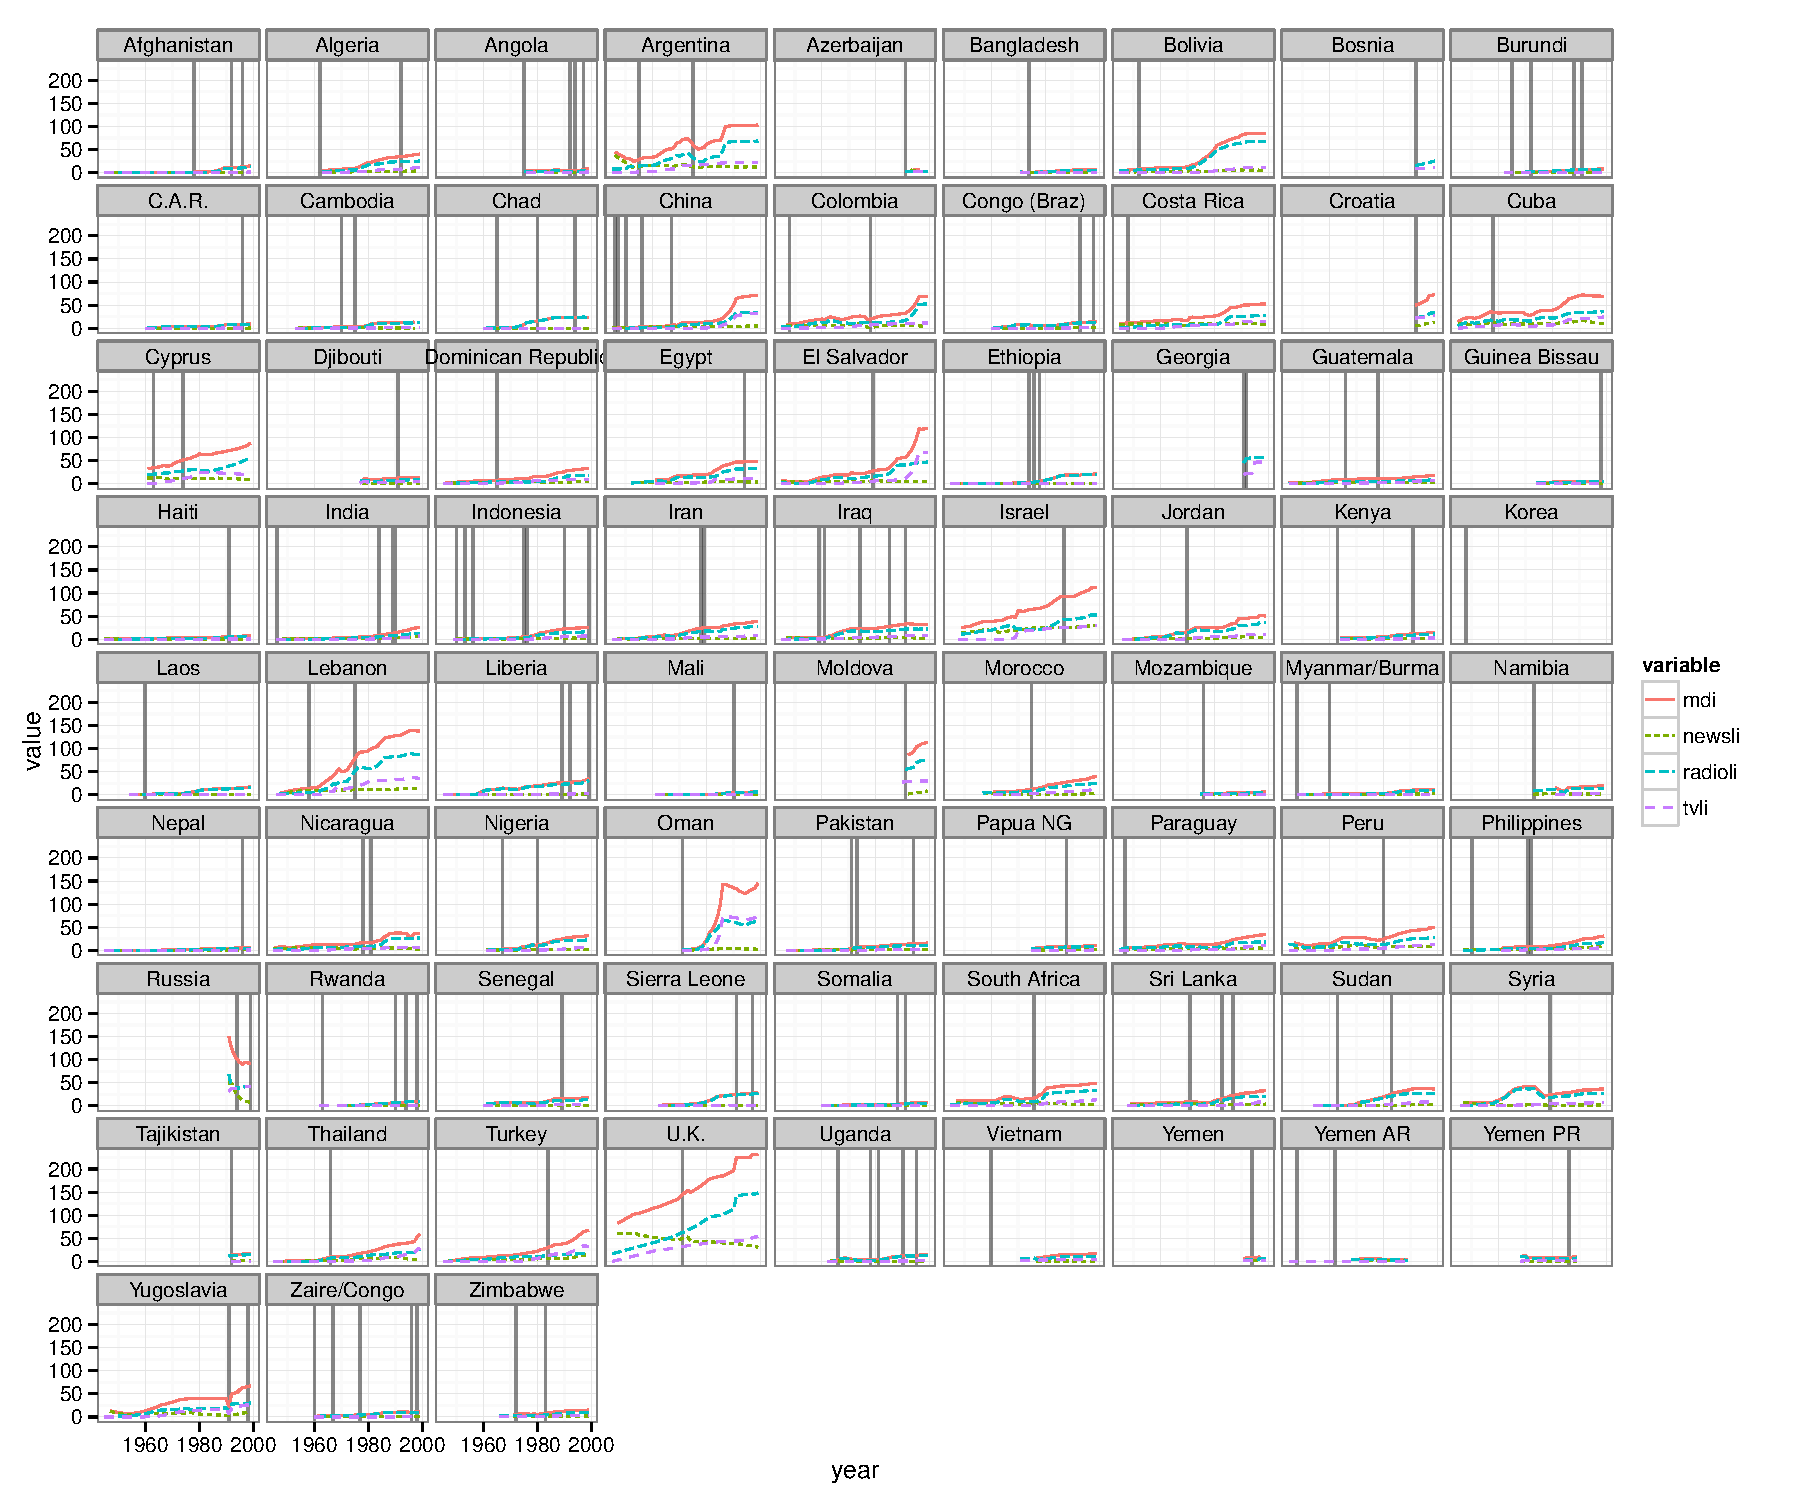
\includegraphics{./media_civil_war_files/figure-markdown/full_panel_plot.pdf}
\caption{Disaggregated media density and all civil war onsets over time,
by country}
\end{figure}

\subsubsection{Tests of Stationarity}\label{tests-of-stationarity}

The Levin-Lin-Chu statistic is a standard test for the presence of a
unit root, otherwise known as non-stationarity or integration of order
I(1), in a time series variable observed across multiple cross-sectional
units. The Im-Pesaran-Shin test is a ``second generation'' test which is
robust to cross-sectional dependence, common in cross-national panel
data. For each test, the null hypothesis is the presence of a unit root.
Because the tests require balanced panels, they were applied only to the
24 countries with the maximum time-series of 55 years, a subset which
still contains significant variation in geography, income, regime type,
and other factors. Specifically, the countries in this subset are:
Canada, Cuba, Haiti, Dominican Republic, Mexico, Honduras, El Salvador,
Nicaragua, Costa Rica, Uruguay, Ireland, Netherlands, Belgium,
Luxembourg, France, Switzerland, Hungary, Romania, Finland, Sweden,
Norway, Denmark, Afghanistan, China.

\begin{verbatim}
Levin-Lin-Chu Unit-Root Test (ex. var. : Individual Intercepts
and Trend )
\end{verbatim}

data: unit\$mdi z.x1 = -0.32, p-value = 0.7473 alternative hypothesis:
stationarity

\begin{verbatim}
Pesaran's CIPS test for unit roots
\end{verbatim}

data: unit\$mdi CIPS test = -2.1, lag order = 2, p-value = 0.1
alternative hypothesis: Stationarity

\subsubsection{Semi-parametric regressions on disaggregated media
density}\label{semi-parametric-regressions-on-disaggregated-media-density}

The following plots display the smoothed terms for each of the
components of MDI, controlling for all the independent variables of the
baseline model and the other components of MDI. All of the components of
MDI are logged before estimation. Each plot was generated by a
semi-parametric regression in which all independent variables are
estimated parametrically except the variable of interest. The dashed
lines represent 95\% confidence bands.

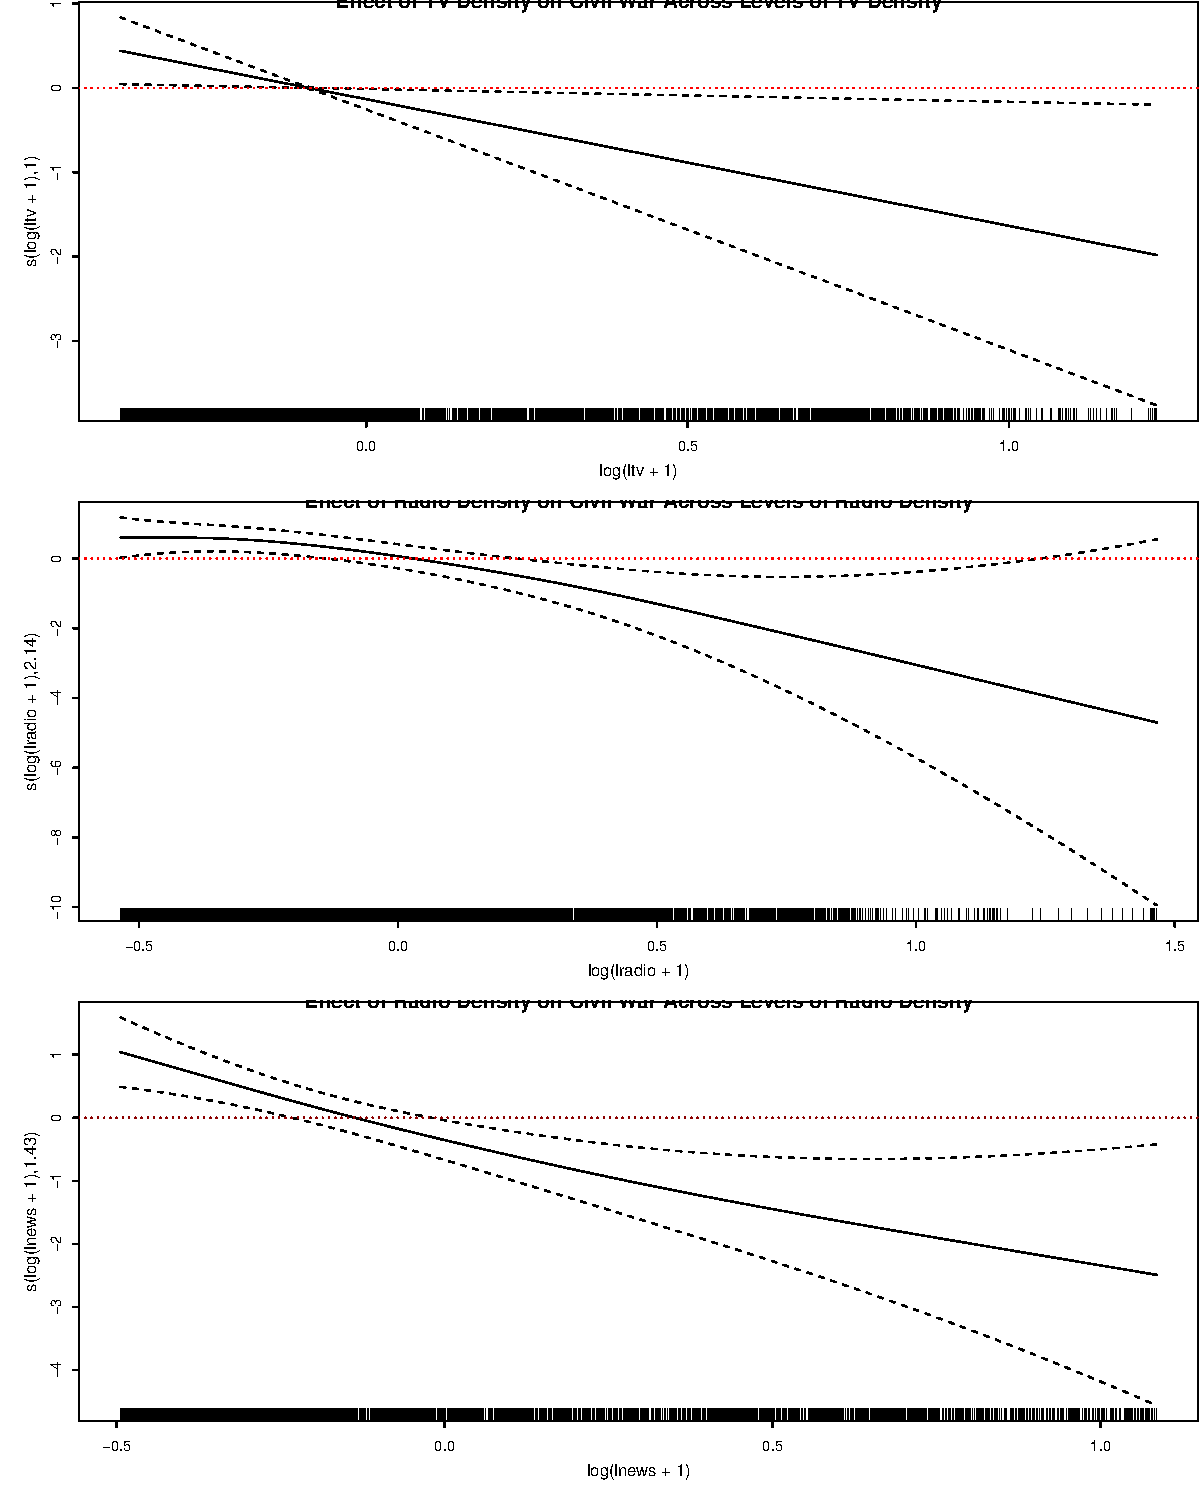
\includegraphics{./media_civil_war_files/figure-markdown/disaggregated-nonlinear.pdf}
\pagebreak   

\section{References}\label{references}

\setlength{\parindent}{-0.2in} \setlength{\leftskip}{0.2in}
\setlength{\parskip}{8pt} \vspace*{-0.2in} \noindent

Anderson, Benedict. 1983. \emph{Imagined Communities: Reflections on the
Origin and Spread of Nationalism}. London: Verso.

Bolt, J. 2013. ``The First Update of the Maddison Project; Re-Estimating
Growth Before 1820.'' \emph{Maddison Project Working Paper} 4.

Deutsch, Karl W. 1953. \emph{Nationalism and Social Communication : an
Inquiry into the Foundations of Nationality}. New York: Technology Press
(M.I.T.).

Fox, John. 2002. ``Nonparametric Regression.'' In \emph{An R and S-Plus
Companion to Applied Regression}, Thousand Oaks, CA.

Fr{ö}lich, Markus. 2006. ``Non-Parametric Regression for Binary
Dependent Variables.'' \emph{Econometrics Journal} 9(3): 511--40.

Hintze, Jerry L, and Ray D Nelson. 1998. ``Violin Plots: A Box
Plot-Density Trace Synergism.'' 52(2): 181--84.

Im, Kyung So, M Hashem Pesaran, and Yongcheol Shin. 2003. ``Testing for
Unit Roots in Heterogeneous Panels.'' \emph{Journal of Econometrics}
115(1): 53--74.

Kastellec, Jonathan P, and Eduardo L Leoni. 2007. ``Using Graphs Instead
of Tables in Political Science.'' \emph{Perspectives on Politics} 5(04):
755--71.

Keohane, Robert O, and Joseph S Nye Jr. 1998. ``Power and
Interdependence in the Information Age.'' \emph{Foreign Affairs} 77(5):
81.

King, G, R O Keohane, and S Verba. 1994. \emph{Designing Social Inquiry:
Scientific Inference in Qualitative Research}. Princeton University
Press.

King, Gary, and Langche Zeng. 2001. ``Logistic Regression in Rare Events
Data.'' \emph{Political Analysis} 9(2): 137--63.

Levin, Andrew, Chien-Fu Lin, and Chia-Shang James Chu. 2002. ``Unit Root
Tests in Panel Data: Asymptotic and Finite-Sample Properties.''
\emph{Journal of Econometrics} 108(1): 1--24.

Nye Jr, Joseph S. 1990. ``Soft Power'' \emph{Foreign Policy} (80):
153--71.

---------. 2004. \emph{Soft Power: The Means to Success in World
Politics}. New York: Public Affairs.

Sambanis, N. 2004. ``What Is Civil War?: Conceptual and Empirical
Complexities of an Operational Definition.'' \emph{Journal of Conflict
Resolution} 48(6): 814--58.

``Scaling Regression Inputs by Dividing by Two Standard Deviations.''
2008. \emph{Statistics in Medicine} 27(15): 2865--73.

Warren, Camber T. 2014. ``Not by the Sword Alone: Soft Power, Mass
Media, and the Production of State Sovereignty.'' \emph{International
Organization} 68(01): 111--41.

Wood, S N. 2000. ``Modelling and Smoothing Parameter Estimation with
Multiple Quadratic Penalties.'' \emph{onlinelibrary.wiley.com} 62(2):
413--28.


\end{document}